\chapter{Interpretation of Search Results Within Theoretical Models}
\label{sec:interpretation}
\section{Introduction}
It is very often the case that a search for \ac{NP} will yield results
consistent with the currently accepted theory (which, in most particle physics
contexts would be the \ac{SM}). In the absence of a discovery\footnote{Certain
  models may also have a role to play in the characterisation of a discovery.},
it is often desirable to provide additional information in the form of a
statistical interpretation of the results. Such an interpretation typically
serves the following goals:
\begin{itemize}
\item Indicate the strength of the analysis in searching for the proposed model
  or set of models. This can then be used as an objective measure by which to
  rank different analyses or to benchmark the progress of a single analysis as
  data is collected.
\item Falsify, to some confidence level, a particular theory or some region of
  parameter space within that theory. In the case of a reasonably generic model,
  parameterised in such a way that it may represent other theories (or
  approximate their experimental signature), theorists may be able to
  test the predictions of a variety of models directly against the results of
  the interpretation. This will be discussed further in Section~\ref{sec:sms}.
\item Guide the optimisation of analysis cuts and object selection.
\end{itemize}

Providing an interpretation invariably necessitates some choice of theory or
phenomenological model against which to test the results. The range of theories
will of course depend strongly on the inclusiveness of the experiment. Indeed,
in many cases a single theory will have motivated the analysis in the first
place and the choice of model will be clear. In other cases, the analysis has
been designed to be as inclusive as possible and therefore sensitive to an array
of theories. Typically this is achieved by focussing on a particular detector
signature (for instance missing transverse energy), where a deviation from the
\ac{SM} is a common feature of many \ac{NP} scenarios.

As was seen in Chapter~\ref{sec:framework}, \ac{LHC} searches have typically
interpreted the results of \ac{SUSY} searches in the context of the
\ac{CMSSM}. This provides a convenient benchmark space for the comparison of
different searches. However, it restricts the range of physics signatures rather
more than is desirable. It was seen that by selecting models from a spectrum of
simplified models, searches can provide more generic and useful interpretations
of their results.

The following chapter will describe the statistical methods used to interpret
the results of the analysis. These will then be applied to the \ac{CMSSM} and to
the two simplified models described previously: \TthreeW and \Ttwott.

\section{Statistical Methods}
\subsection{The Likelihood Function}
Consider some statistical model believed to describe a set of experimental data
and dependent on a set of parameters, $\theta$. The likelihood for given values
of $\theta$ and given a set of experimental observations $X$, is the probability
of observing $X$ given $\theta$~\cite{statistical_methods}. Considered as a
function of the parameter $\theta$ given experimental measurements, $X$, the
likelihood may be written
\begin{equation}
\likelihood\left(\theta|X\right) = P\left(X|\theta\right)
\label{eqn:inter_likelihood}
\end{equation}
where $P\left(X|\theta\right)$ should be read as ``the probability of $X$ given
$\theta$''.

Likelihood functions are an important tool in comparing theoretical expectations
to experiment. Often, two proposed values for the parameter $\theta$ will be
compared using the \emph{likelihood ratio},
\begin{equation}
  \likelihoodratio = \frac{\likelihood\left(\theta_1|X\right)}{\likelihood\left(\theta_2|X\right)} = \frac{\alpha P\left(X|\theta_1\right)}{\alpha P\left(X|\theta_2\right)}
\label{eqn:inter_likelihood_ratio}
\end{equation}
Here, the numerator and denominator are related to
Eqn~\ref{eqn:inter_likelihood} by a constant $\alpha$. Here, as in many uses of
the likelihood function, such constant factors can be safely ignored.  This is
known as a \emph{likelihood ratio test} and may be used to compare two
hypotheses.

An important use of the likelihood function is in estimation of the parameters
$\theta$ given some set of observations. The value of $\theta$ which maximises
$\likelihood$ is known as the \acl{MLE} of $\theta$, denoted
$\hat{\theta}$. Often it will be convenient to work with the logarithm of the
likelihood function, $\ln\likelihood$. Since the logarithm is a monotonically
increasing funtion, its maxima coincide with the maxima of $\likelihood$.


\subsection{Profile Likelihood and Wilk's Theorem}
\label{sec:inter_profile_likelihood}
The likelihood function for a complex experiment may depend on a large number of
free parameters. A number of these may be introduced to describe experimental
effects such as backgrounds or uncertainties which are not directly relevant to
the underlying measurement. These are known as \emph{nuisance parameters}. The
parameters to be measured by the experiment are known as \emph{parameters of
  interest}.

The full likelihood function may be reduced to a ``profile likelihood'', by
rewriting the nuisance parameters in terms of the parameters of interest. For
instance, the profile likelihood ratio,
\begin{equation}
  \lambda = \frac{\likelihood\left(\mu, \hat{\hat{\nu}}\left(\mu\right)\right)}{\likelihood\left(\hat{\mu}, \hat{\nu}\right)}
\end{equation}
where $\mu$ are the parameters of interest and $\nu$ the nuisance
paramters. $\hat{\mu}$ and $\hat{\nu}$ are the \acp{MLE} of $\mu$ and $\nu$
respectively. $\hat{\hat{\nu}}$ is the \emph{conditional} \ac{MLE} of $\nu$ -
the maximum likelihood estimator of $\nu$ for a given value of $\mu$.

It is frequently the case that, in addition to calculating a maximum-likelihood
estimate for a given parameter, it is also desirable to estimate an interval in
which the ``true'' value of the parameter can be said to lie with a given degree
of certainty. This is known as \emph{interval estimation}.

Wilk's theorem states that $-2\ln\likelihoodratio$ is distributed as a $\chi^2$
distribution. The number of degrees of freedom of this distribution is
determined by the difference in the number of free parameters in the numerator
and denominator of the likelihood ratio ($\theta_1$ and $\theta_2$ in
Eqn~\ref{eqn:inter_likelihood_ratio}). In the case of the profile likelihood
ratio, this is equal to the number of parameters of interest, $\mu$. Wilk's
theorem can therefore be used to provide an interval estimate for the parameters
of interest $\mu$. This method will be referred to in the sequel as the \ac{PL}
method.

\subsection{Hypothesis Testing}
\label{sec:inter_cls}
It has been seen that the likelihood ratio may be used to compare two hypotheses
$H_0$ and $H_1$. Typically $H_0$ will be referred to as the ``null hypothesis''
and $H_1$, the ``alternate hypothesis''. For a given hypothesis $H$ and having
made a certain observation $X$, the \emph{p-value} gives the probability of
making a measurement as consistent or less with the hypothesis $H$ than the data
actually observed, $X$.

There are a variety of techniques for choosing between competing
hypotheses. Typically, a certain test statistic is used - for instance the
number of signal events observed or the likelihood ratio. For a given
hypothesis, a critical region $W$ can be defined where the probility of measuring
such a value given the hypothesis is below some threashold,
\begin{equation*}
P\left(x \in W|H\right) \leq \alpha
\end{equation*}
where $x$ is the test statistic and $\alpha$ is some small constant - normally
$0.05$. If the measured value of $x$ is found to be in the critical region, the
hypothesis $H$ can be said to be rejected with 95\% confidence.

One way to define such an interval is to run toy Monte Carlo experiments to
generate the distributions of the test statistic corresponding to the null and
alternate hypotheses. It is then straightforward to define the critical region
as that point at which the p-value reaches a suitably low threshold, say
$0.05$. This is illustrated in Figure~\ref{fig:inter_cls_explain1}.

\begin{figure}
\centering
\subfloat[]{\label{fig:inter_cls_explain1}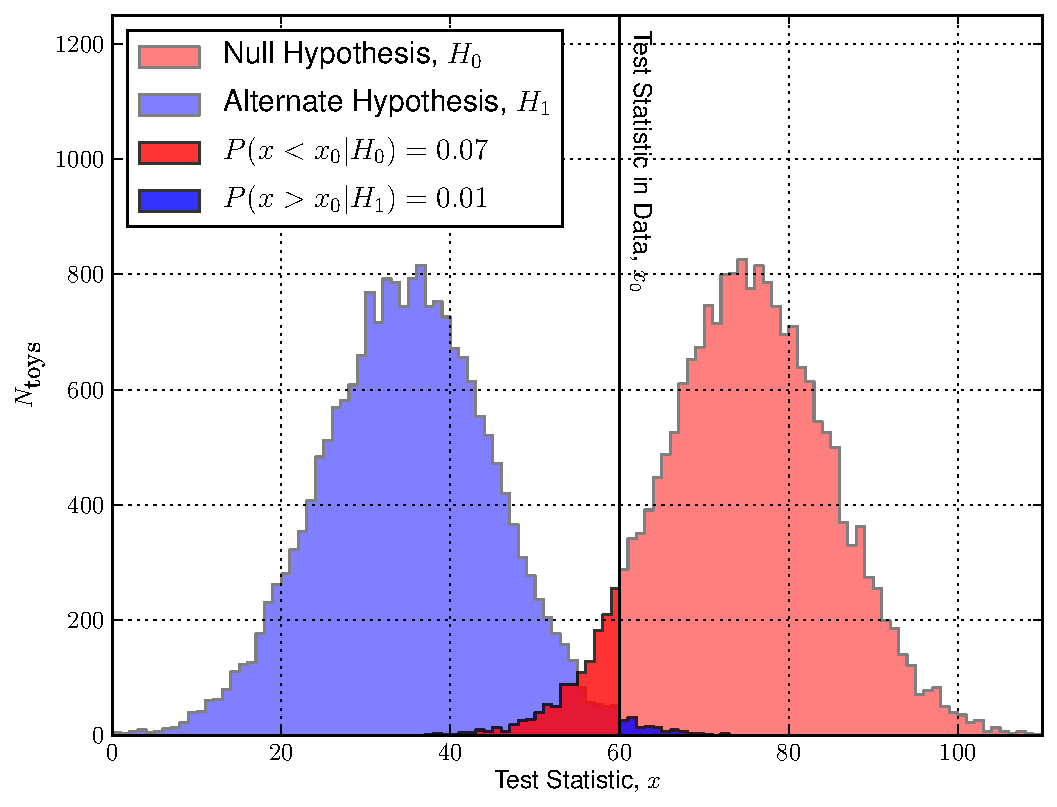
\includegraphics[width=0.49\textwidth]{fig/cls1}}
\subfloat[]{\label{fig:inter_cls_explain2}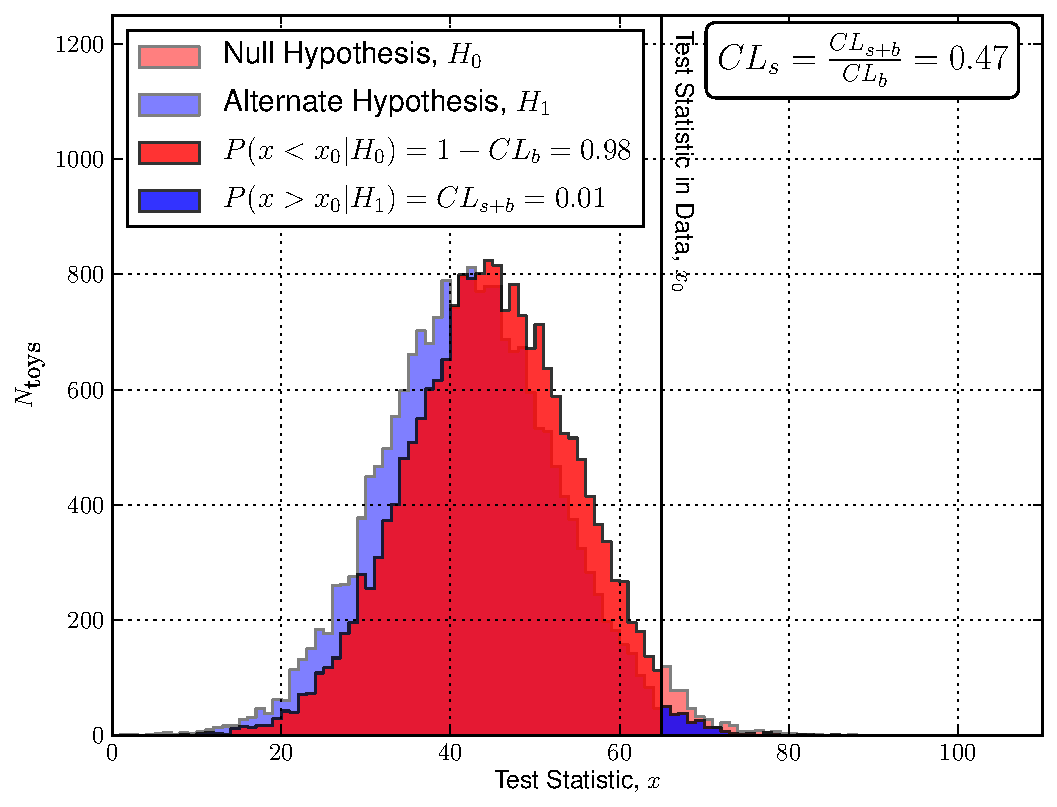
\includegraphics[width=0.49\textwidth]{fig/cls2}}
\caption[]{}
\label{fig:inter_cls_explain}
\end{figure}

\subsection{The \CLs Method}
One deficiency of the above method is that often the two hypotheses will not be
so well separated. This situation is shown in
Figure~\ref{fig:inter_cls_explain2}. In this case, the p-value for the alternate
hypothesis is small and so would result in an exclusion. This is undesirable
since the test statistic is clearly not sensitive enough to distinguish between
the two hypotheses.

To address this problem, the \CLs hypothesis test may be used instead~\cite{cls},
\begin{equation*}
\CLs = \frac{CL_{s+b}}{CL_{b}}
\end{equation*}
where, for the example shown in Figure~\ref{fig:inter_cls_explain2},
\begin{eqnarray*}
CL_{s+b} = P\left(x > x_0 | H_1\right)\\
CL_b = 1 - P\left(x < x_0 | H_0\right)
\end{eqnarray*}
where the null hypothesis now represents a background-only ($b$) scenario, and
the alternate, signal-plus-background ($s+b$). Using the \CLs to test the
alternate hypothesis, instead of a p-value, penalises cases where the test
statistic provides little sensitivity - since $CL_b$ will be large. For a 95\%
exclusion, $\CLs < 0.05$ is required, as before. The \CLs method may also be
used to derive an upper limit on some parameter by scanning through different
values of the parameter of interest in order to obtain a 95\% upper limit. This
is known as ``hypothesis test inversion''.

Several additional details are relevant to the discussion here. For the toy
experiments used to generate the test statistic distributions, the nuisance
parameters are each sampled randomly according to their expected
distributions. This ensures that the full range of their uncertainties is
covered. The test statistic that has been used is the one-sided profile
likelihood ratio, $\qmu=-2\ln\lambda$~\cite{cl_computation,
  modified_frequentist, atlas_cms_higgs}.

\section{The Single Lepton Supersymmetry Search}
The full development of the likelihood function used to model the single lepton
supersymmetry search is covered in complete detail in
Appendix~\ref{sec:inter_1lepton}. In this section, only a few pertinent points
will be discussed. Firstly, the evaluation of model-dependent systematic effects
associated with the signal yield. Secondly, some discussion of validation work
performed to demonstrate that the statistical procedure and software
infrastructure are functioning as expected.

\subsection{Signal Systematics}
As can be seen in Table~\ref{tbl:inter_systematic_parameters}, a number of
nuisance parameters are assigned for systematic uncertainties affecting the
expected signal yield.

Both the luminosity estimate and the trigger efficiency are subject to
uncertainties which would effect the expected signal yield. Uncertainties of 4\%
and 1\% are assigned.

The signal efficiency will also be affected by the choice of \acp{PDF} in the
simulated samples and the calculation of the \ac{NLO} cross-sections. Whilst in
principal these would be expected to vary across the parameter space of a given
theoretical model, the complexity of the calculation involved in accurately
evaluating this systematic led us to assign a conservative 10\% systematic.

For the jet energy scale and \MET resolution uncertainty, these are calculated
as for the background case (see Sections~\ref{sec:susy_jes_uncertainty} and
\ref{sec:susy_metres_uncertainty}). These are calculated individually for
different signal hypotheses. As summary of all uncertainties assigned for the
signal efficiencies, along with their exact or approximate size, is shown in
Table~\ref{tbl:inter_signal_systematics}.

\ctable[
caption=Summary table of uncertainties related to the signal efficiency.,
mincapwidth=0.5\textwidth,
label=tbl:inter_signal_systematics,
pos=h
]{cc}{
}{\FL
Uncertainty & Value\ML
$\mathcal{L}$ & 4.5\%\NN
trigger efficiency & 1\%\NN
JES 5\% & Model dependent (10-15\% for \ac{CMSSM})\NN
PFMET resolution 10\%& Model dependent (0.5-15\% for \ac{CMSSM})\NN
PDF and NLO& 10\%\LL
}


\begin{figure}[h!]
\centering
\subfloat[]{\label{fig:inter_pl_80_400_syst}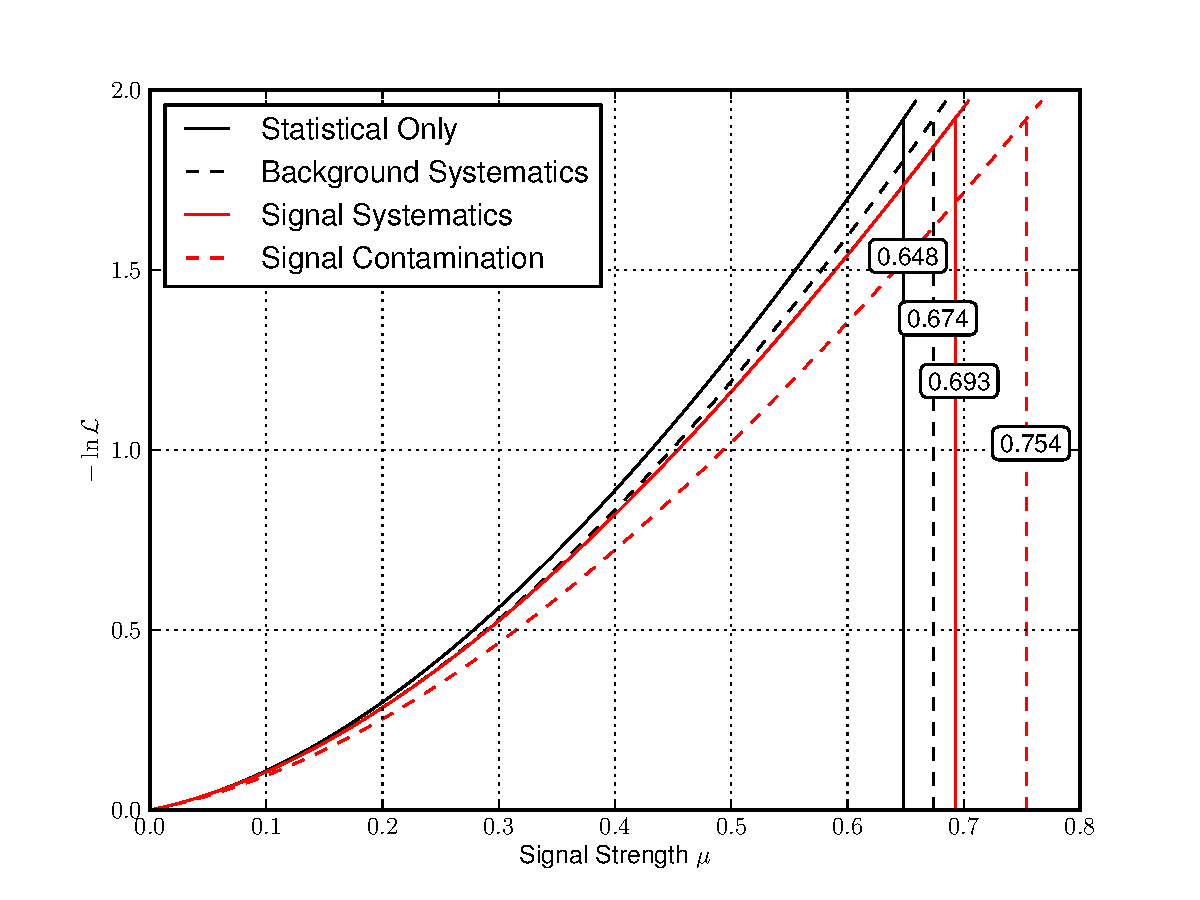
\includegraphics[width=0.47\textwidth]{fig/pl_systematics_80_400}}\quad
\subfloat[]{\label{fig:inter_pl_80_400_muon}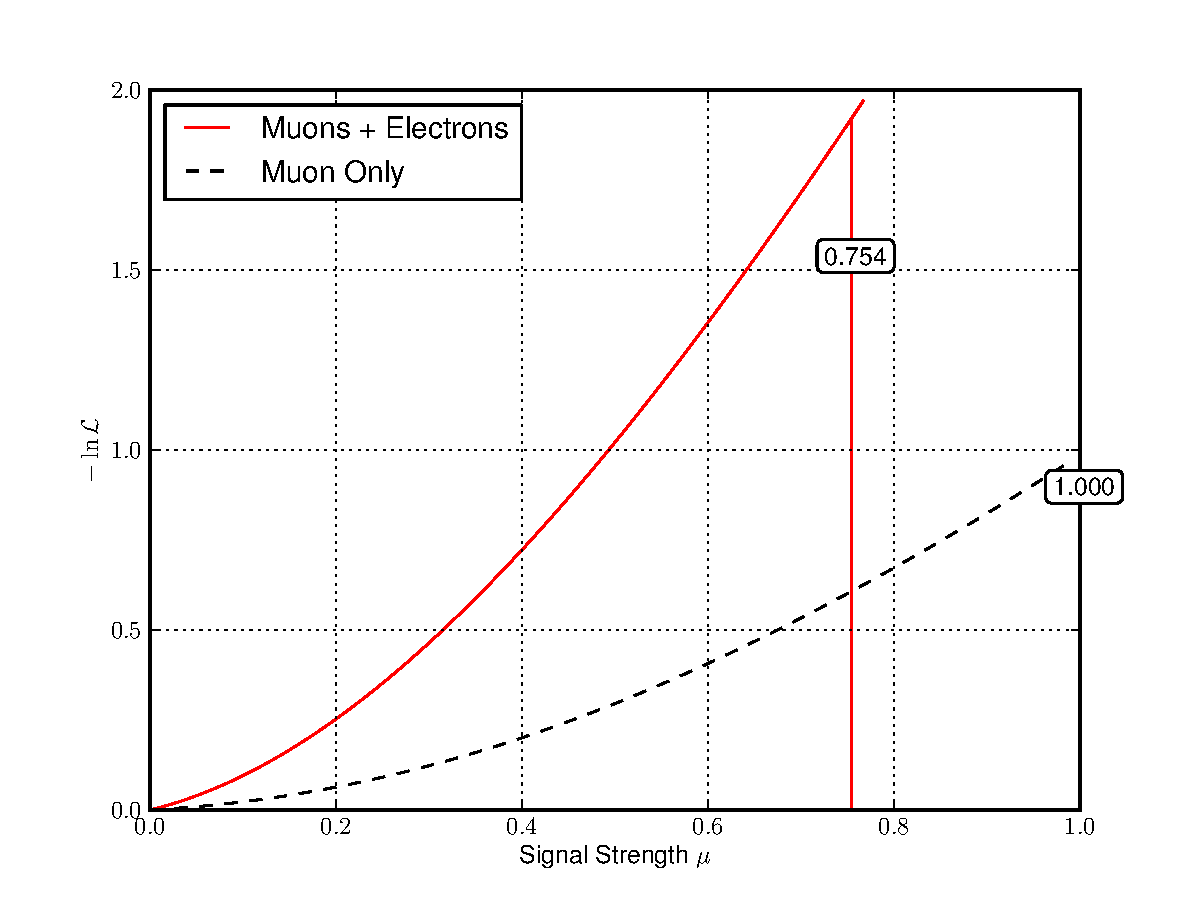
\includegraphics[width=0.47\textwidth]{fig/pl_muon_80_400}}
\caption{Comparison of the shape of the profile likelihood function with
  different systematic effects included at the \ac{CMSSM} point $(\Mzero, Mhalf)
  = (80, 400)$}
\label{fig:inter_pl}
\end{figure}

\begin{figure}[h!]
\centering
\subfloat[Statistical Uncertainties Only]{
  \label{fig:inter_cls_80_400_syst}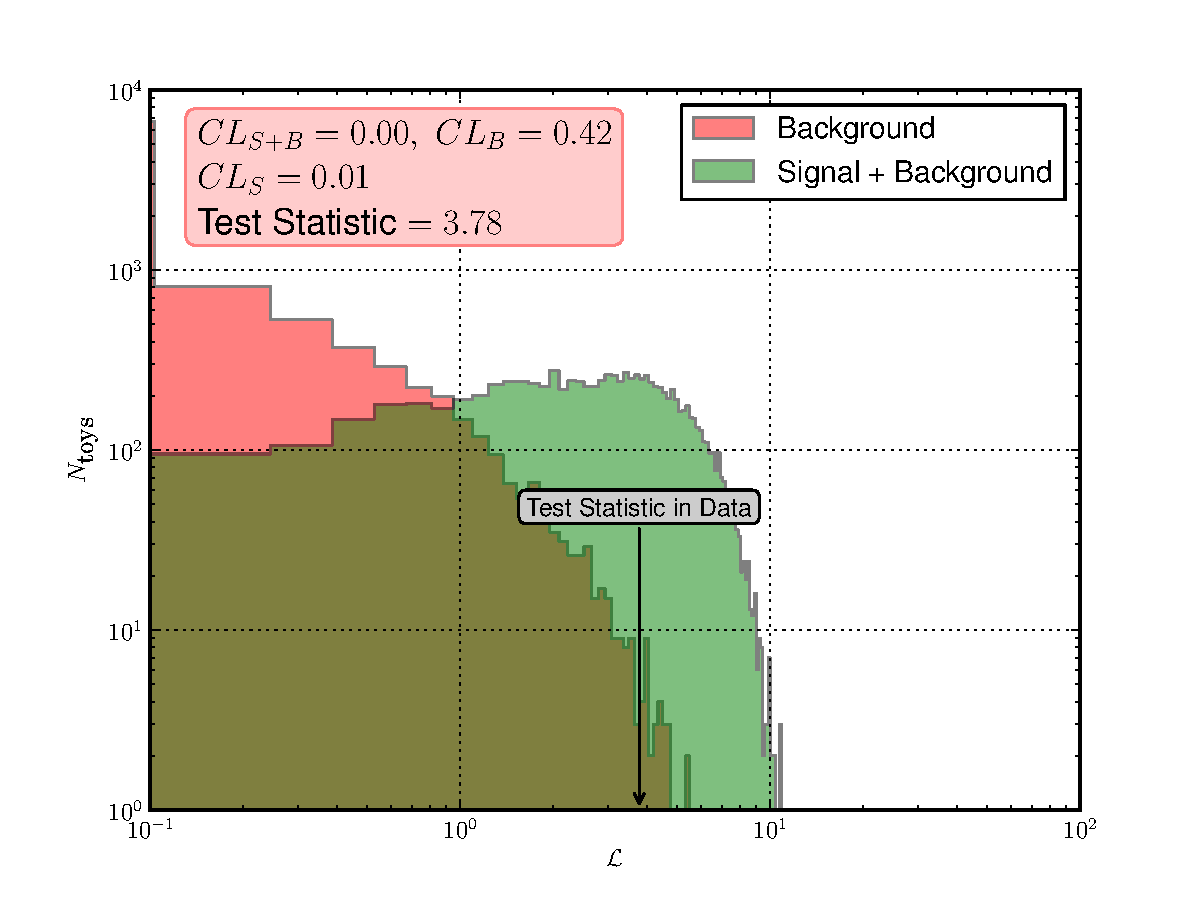
\includegraphics[width=0.47\textwidth]{fig/exp_muon_electron_80_400_bgsysts_no_sigsysts_no_sigcon_no}}\quad
\subfloat[Background Systematics]{
  \label{fig:inter_cls_80_400_muon}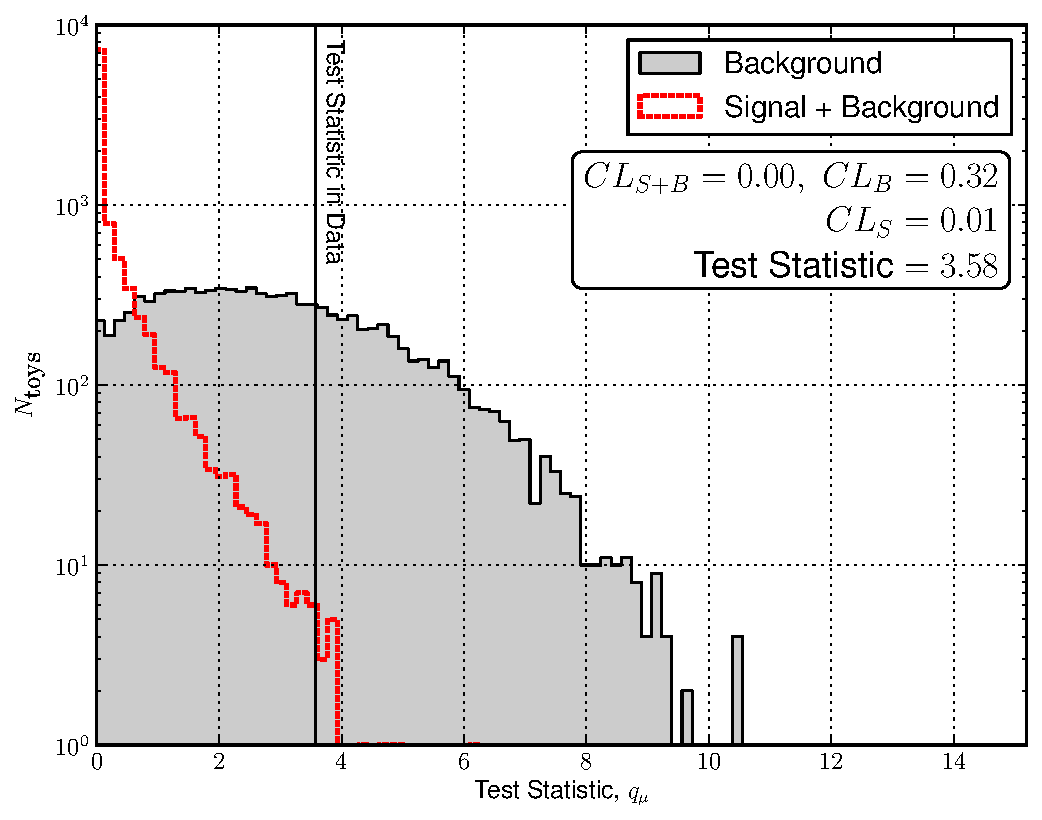
\includegraphics[width=0.47\textwidth]{fig/exp_muon_electron_80_400_bgsysts_yes_sigsysts_no_sigcon_no}}\\
\subfloat[Signal Systematics]{
  \label{fig:inter_cls_80_400_syst}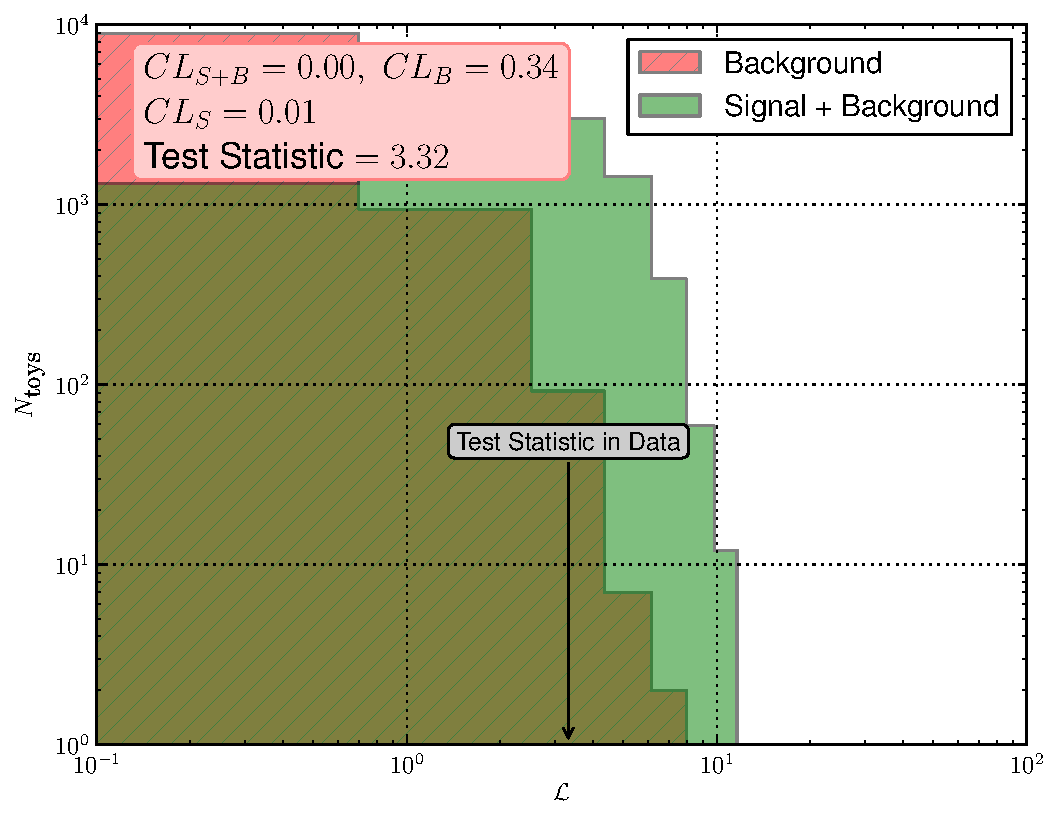
\includegraphics[width=0.47\textwidth]{fig/exp_muon_electron_80_400_bgsysts_yes_sigsysts_yes_sigcon_no}}\quad
\subfloat[Signal Contamination]{
  \label{fig:inter_cls_80_400_muon}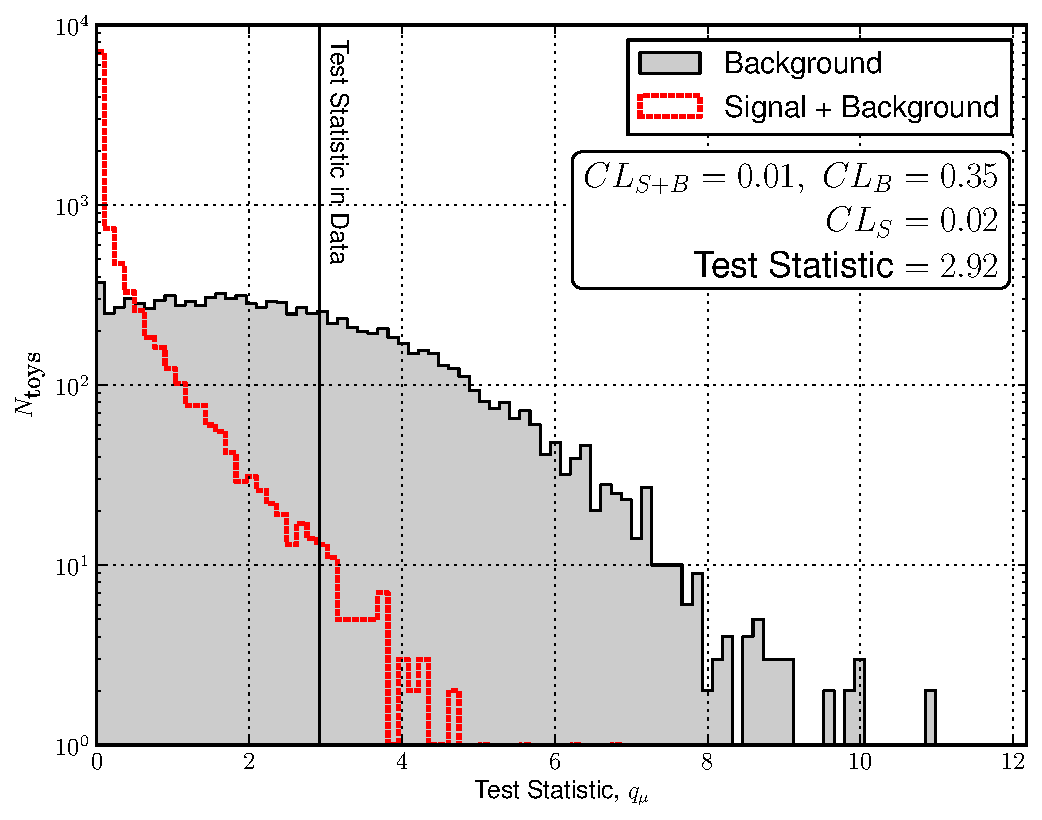
\includegraphics[width=0.47\textwidth]{fig/exp_muon_electron_80_400_bgsysts_yes_sigsysts_yes_sigcon_yes}}\\
\subfloat[Muon Channel Only]{
  \label{fig:inter_cls_80_400_muon}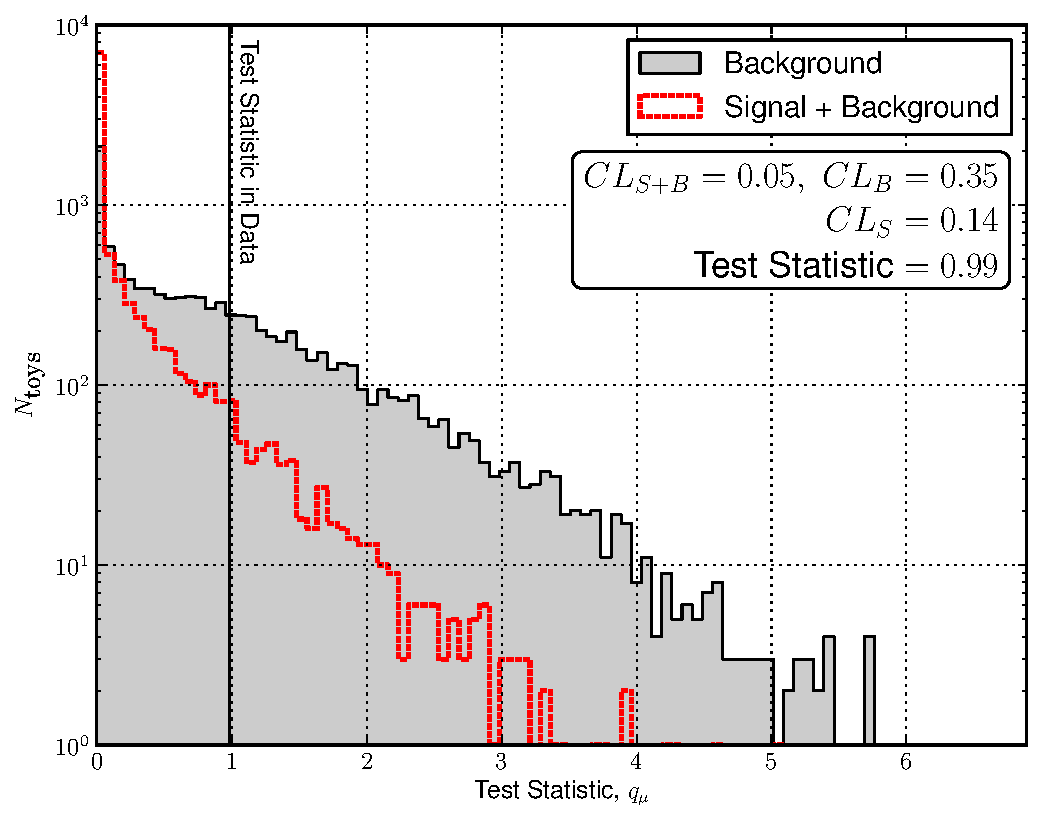
\includegraphics[width=0.47\textwidth]{fig/exp_muon_80_400_bgsysts_yes_sigsysts_yes_sigcon_yes}}
\caption[Distribution of the profile likelihood ratio test statistic for null
and alternate hypotheses with different systematic effects
included]{Distribution of the profile likelihood ratio test statistic for null
  and alternate hypotheses with different systematic effects included. These
  distributions have been made for the \ac{CMSSM} point $(\Mzero, \Mhalf) = (80,
  400)$. The values of \CLb, \CLspb and \CLs are also shown.}
\label{fig:inter_cls}
\end{figure}

\subsection{Validation}
\label{sec:inter_validation}
To validate the correct working of the model, a number of cross-checks were
performed. Firstly, the Profile Likelihood and \CLs methods were compared and
found to agree. In general, the \CLs method is expected to be more conservative
in convering the full range of the nuisance parameters in the model.

To see how the Profile Likelihood and \CLs results change with modifications to
the likelihood function, a representative point in the \ac{CMSSM} plane
($\tan\beta=10$, $A_0=0$, $\mu>0$) has been chosen. This is $(m_0,
m_{\frac{1}{2}}) = (80, 400)$, close to the edge of the region excluded by data
(additional detail can be found in Appendix~\ref{sec:app_inter_validation}).

The Profile Likelihood function for this point can be seen in
Figure~\ref{fig:inter_pl}. It can be seen that adding the various systematic
effects to the model, and also removing the electron channel appear to worsen
the exclusion. This shows, qualitatively at least, that the model is behaving as
expected. For this particular model point, the signal contamination appears to
have the largest effect, followed by the background uncertainties and then the
signal uncertainties. Note that certain uncertainties are included in all cases:
the effect of limited statistics in the control region, and the luminosity
uncertainty. Since the former is actually the dominant uncertainty on the
background prediction, this perhaps explains why it appears to have a relatively
small effect.

The distributions of the test statistic used to calculate \CLs are shown in
Figure~\ref{fig:inter_cls}. Again the effect of introducing additional
systematic parameters and removing the electron channel causes \CLs to
increase. This particular point goes from being strongly excluded at $> 95\%$
confidence level with both lepton channels, to not being excluded when the
electrons are removed.

\section{Results}
The likelihood model is used to provide interpretation within the context of two
\ac{NP} models: \ac{CMSSM} and the \Ttwott simplified model described in
Section~\ref{sec:sms}.

\begin{figure}[h!]
\centering
\subfloat[$250 < \STlep < 350$]{\label{fig:inter_msugra_mu_eff250}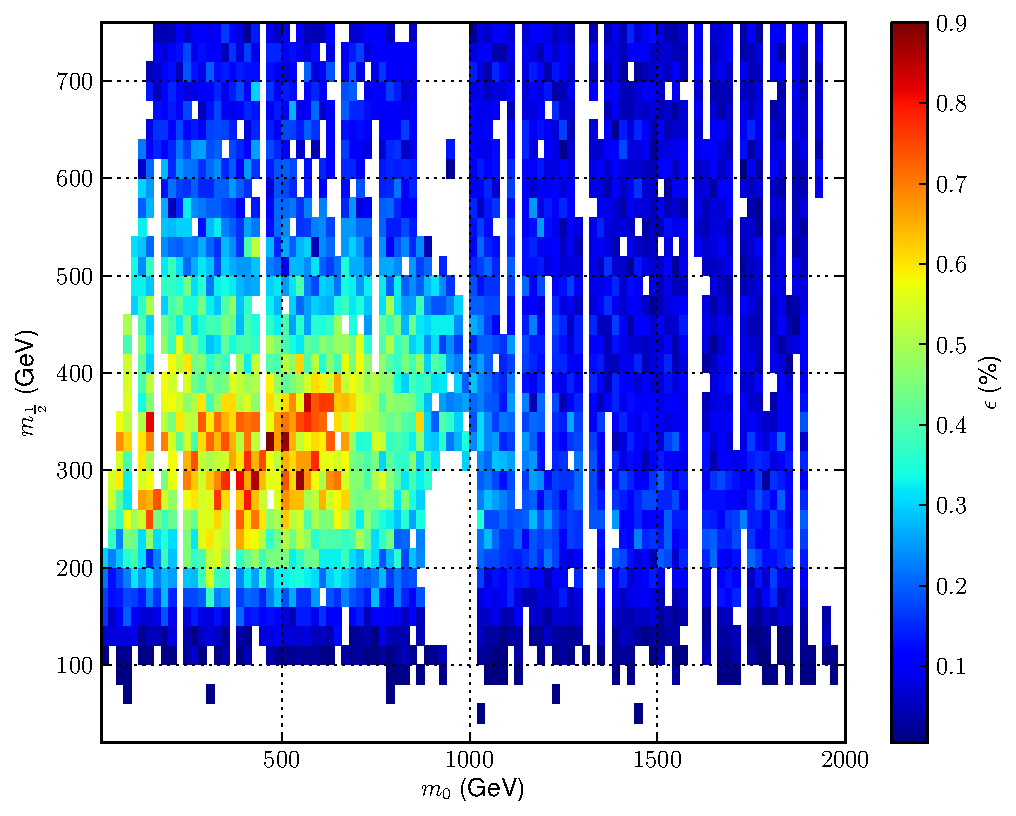
\includegraphics[width=0.49\textwidth]{fig/msugra_muons_eff_250}}
\subfloat[$350 < \STlep < 450$]{\label{fig:inter_msugra_mu_eff350}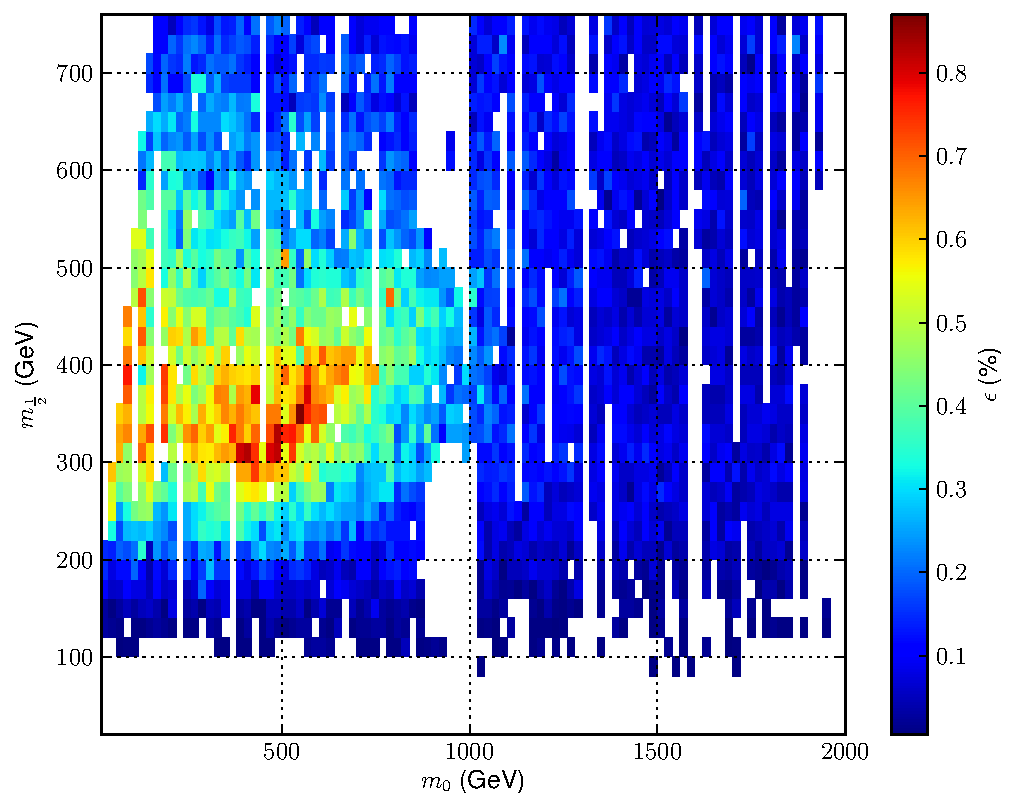
\includegraphics[width=0.49\textwidth]{fig/msugra_muons_eff_350}}\\
\subfloat[$\STlep > 450$]{\label{fig:inter_msugra_mu_eff450}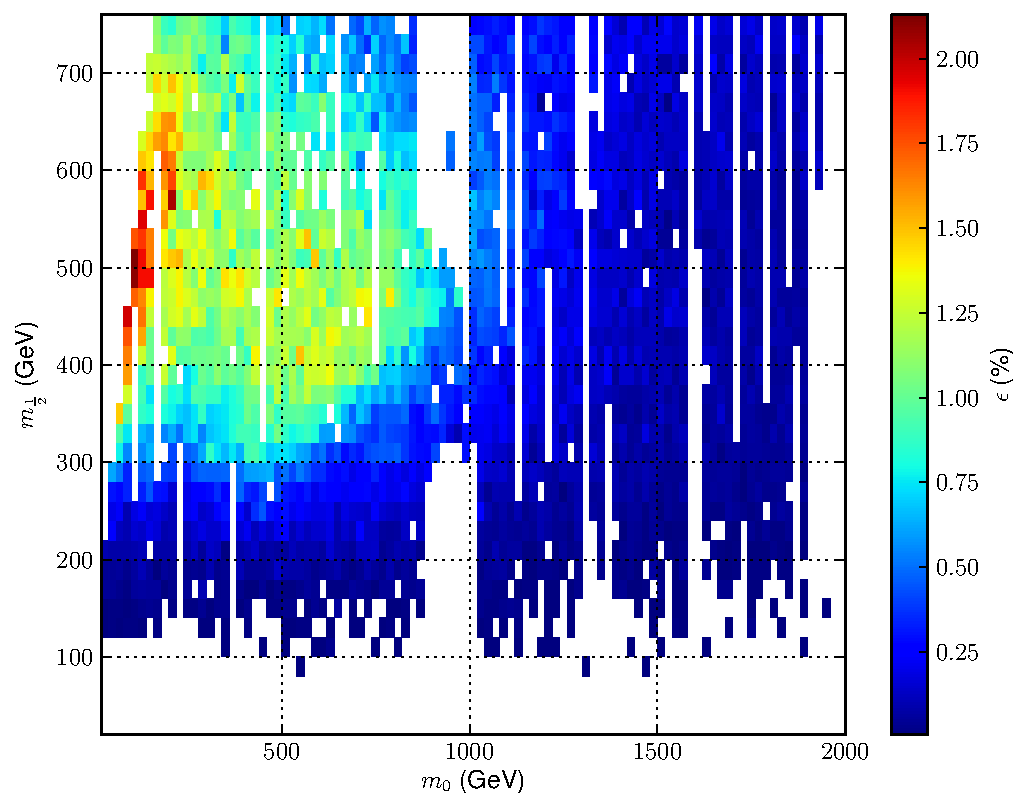
\includegraphics[width=0.49\textwidth]{fig/msugra_muons_eff_450}}
\subfloat[Total]{\label{fig:inter_msugra_mu_efftot}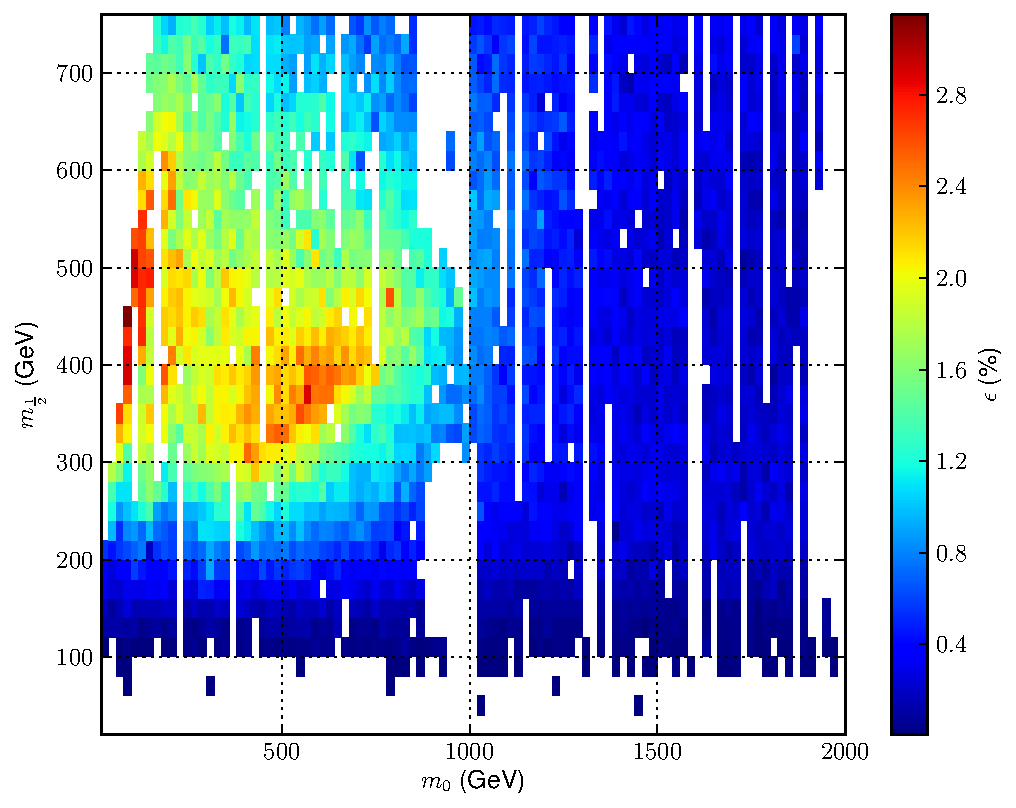
\includegraphics[width=0.49\textwidth]{fig/msugra_muons_eff_total}}
\caption[Signal efficiency for the muon channel in the \ac{CMSSM}]{Signal
  efficiency for the muon channel in the \ac{CMSSM}. The efficiency is shown
  separately for each \STlep bin and as a total. The efficiency is shown in the
  $(\Mzero, \Mhalf)$ plane with $\tanbeta=10$, $\Azero=0$ and $\mu > 0$.}
\label{fig:inter_msugra_mu}
\end{figure}

\begin{figure}[h!]
\centering
\subfloat[$250 < \STlep < 350$]{\label{fig:inter_msugra_el_eff250}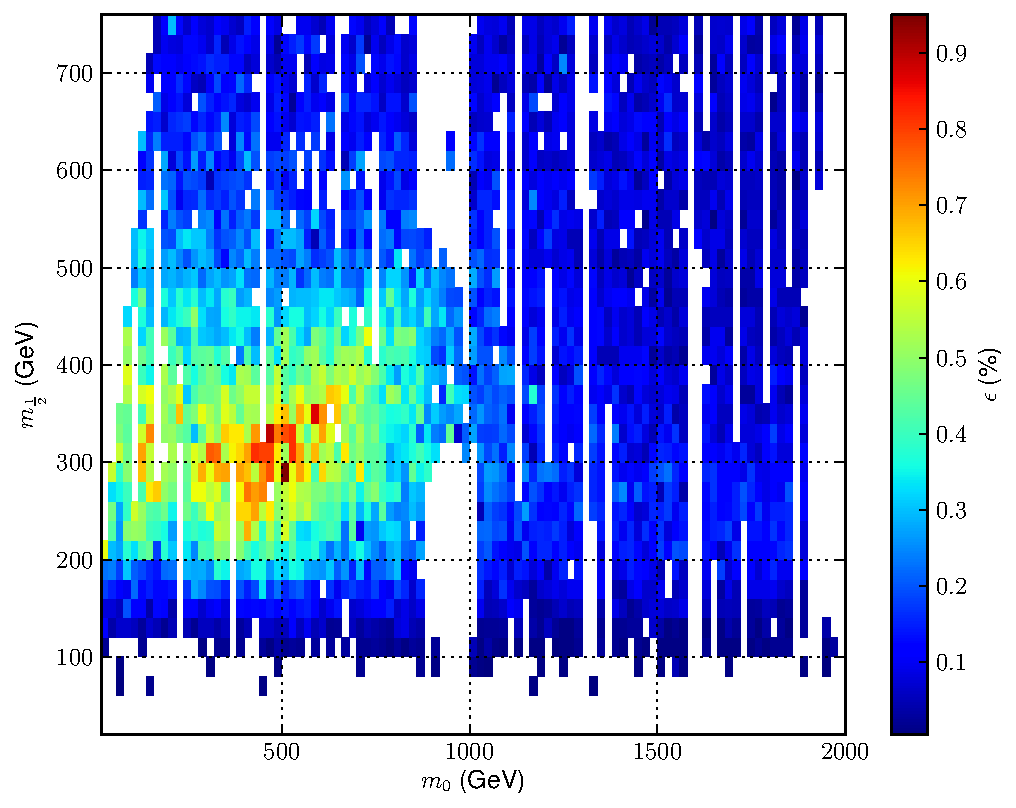
\includegraphics[width=0.49\textwidth]{fig/msugra_electrons_eff_250}}
\subfloat[$350 < \STlep < 450$]{\label{fig:inter_msugra_el_eff350}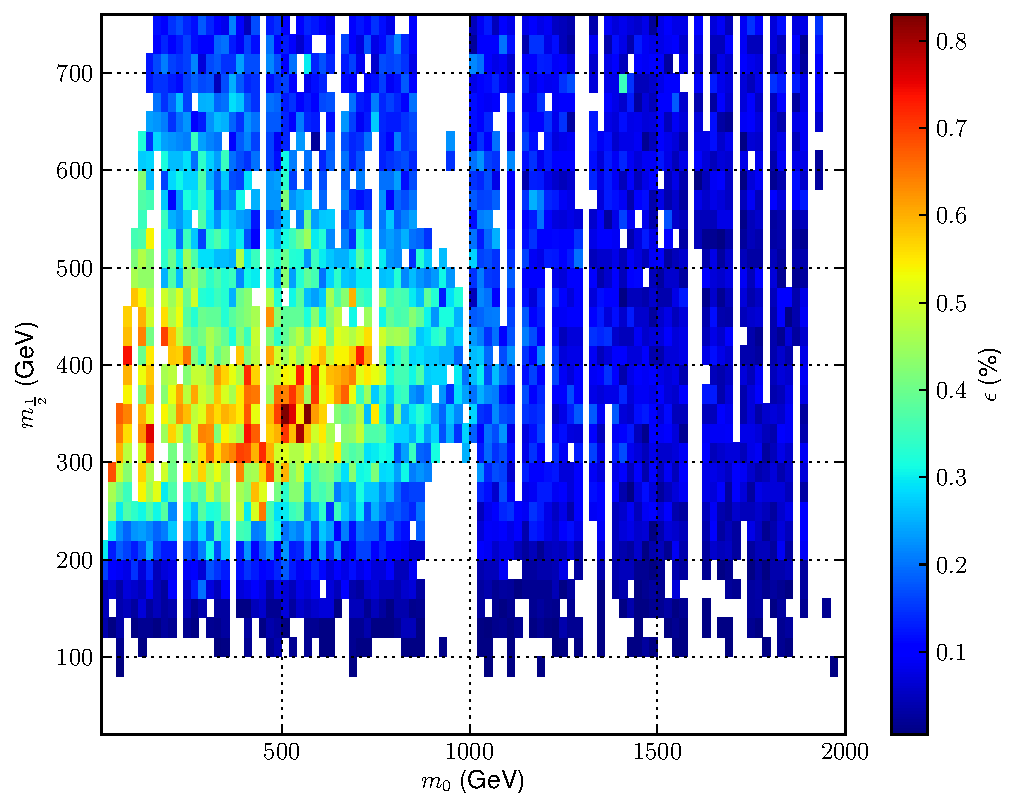
\includegraphics[width=0.49\textwidth]{fig/msugra_electrons_eff_350}}\\
\subfloat[$\STlep > 450$]{\label{fig:inter_msugra_el_eff450}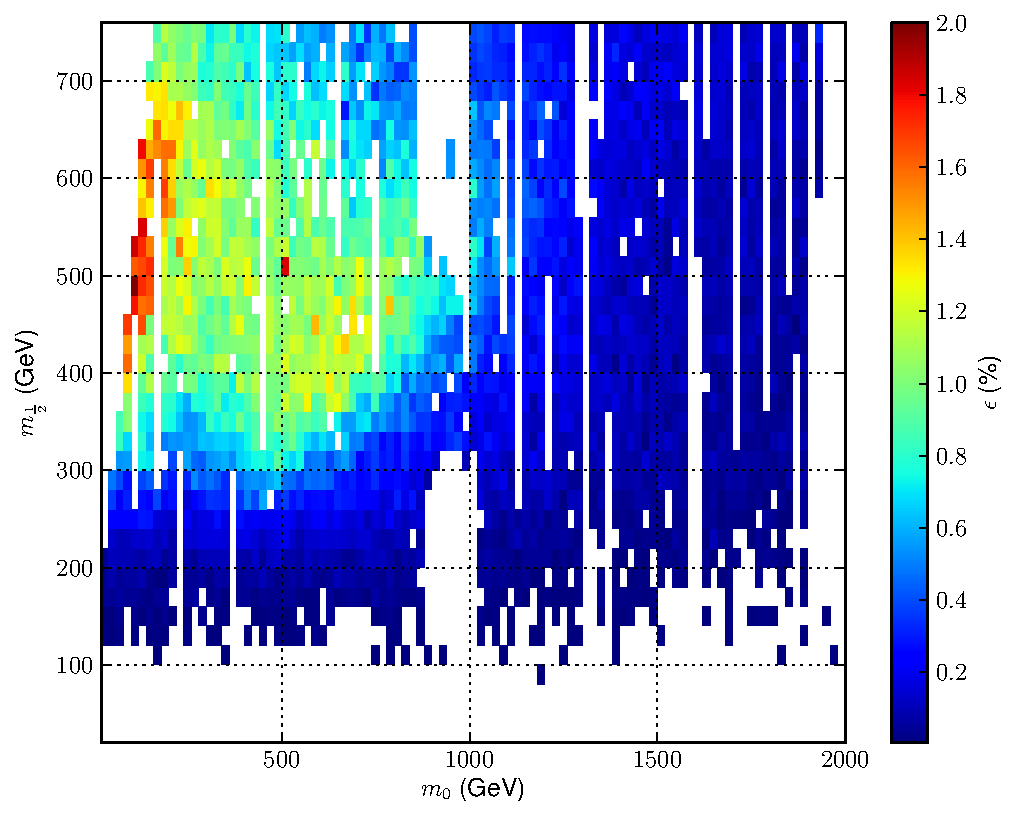
\includegraphics[width=0.49\textwidth]{fig/msugra_electrons_eff_450}}
\subfloat[Total]{\label{fig:inter_msugra_el_efftot}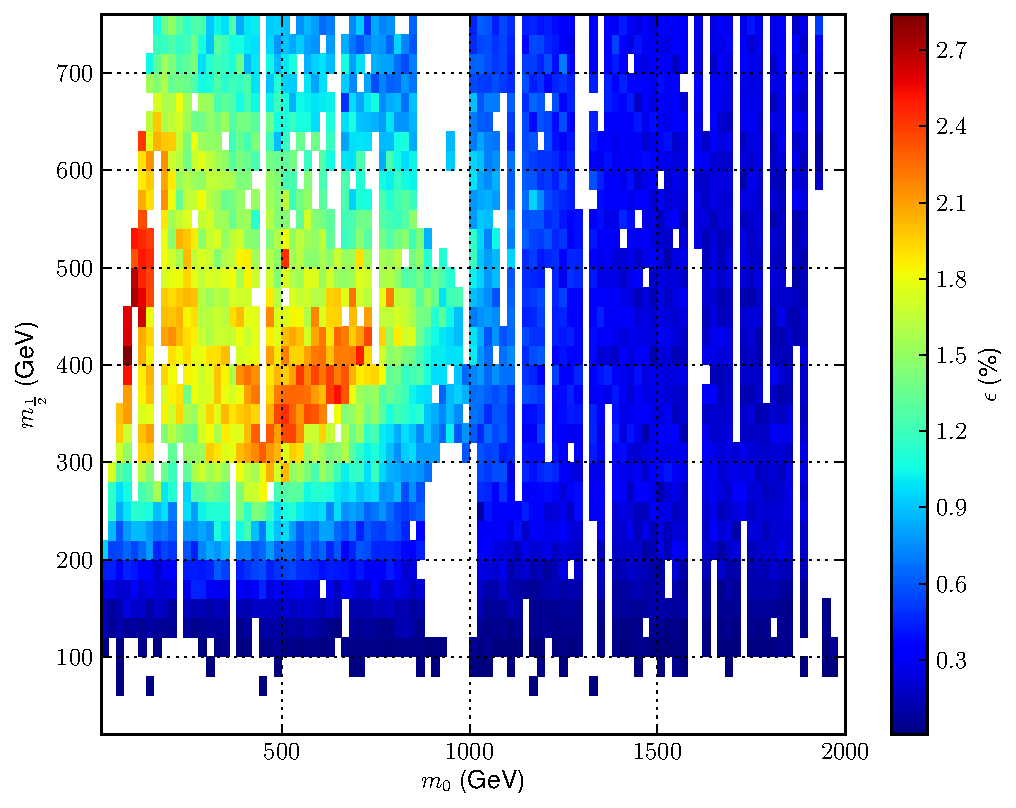
\includegraphics[width=0.49\textwidth]{fig/msugra_electrons_eff_total}}
\caption[Signal efficiency for the electron channel in the \ac{CMSSM}]{Signal
  efficiency for the electron channel in the \ac{CMSSM}. The efficiency is shown
  separately for each \STlep bin and as a total. The efficiency is shown in the
  $(\Mzero, \Mhalf)$ plane with $\tanbeta=10$, $\Azero=0$ and $\mu > 0$.}
\label{fig:inter_msugra_el}
\end{figure}

\begin{figure}[h!]
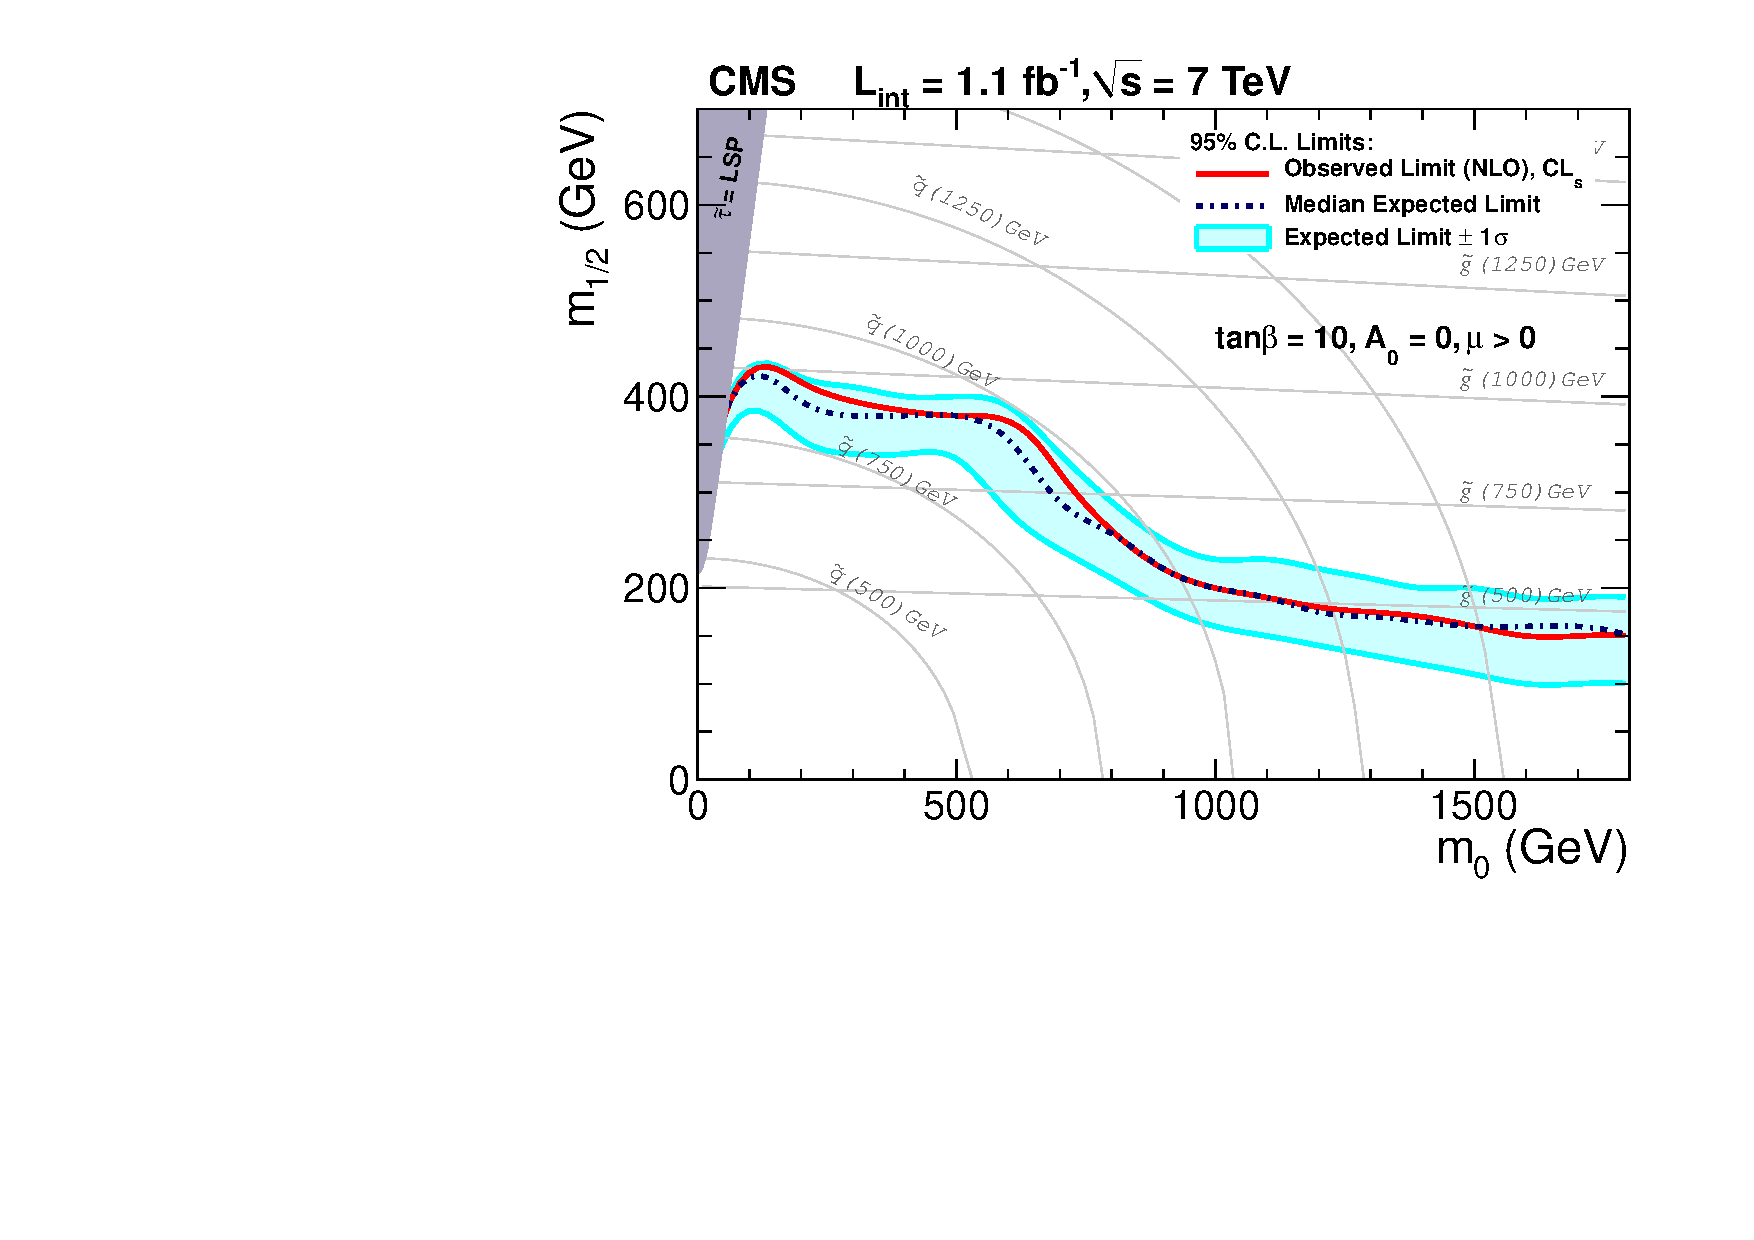
\includegraphics[width=\textwidth]{fig/RA4_ExclusionLimit_tanb10}
\caption[95\% confidence level exclusion plot for the \ac{CMSSM}]{95\% confidence level exclusion plot for the
  \ac{CMSSM}. Shown are the observed (red), expected (blue dotted) and $\pm
  1\sigma$ exclusion bands (light blue shaded) as calculated using the \CLs
  method. Lines of constant squark and gluino mass are also shown.}
\label{fig:inter_msugra_exclusion}
\end{figure}

\subsection{\ac{CMSSM}}
The \ac{CMSSM} was previously described in Section~\ref{sec:cmssm}. As explained
previously, the \ac{CMSSM} makes a number of somewhat arbitrary choices which
restrict the \ac{SUSY} toplogies signatures it is able to encompass. Whilst
these make it relatively undesirable as a framework for theoretical
interpretation, it is nonetheless useful as a common yardstick by which to
compare experiments and searches.

The \ac{CMSSM} results are presented as a 95\% exclusion in a two-dimensional
plane of the parameter space where the two mass parameters, \Mzero and \Mhalf,
are allowed to vary. Other parameters are fixed as follows: $\Azero = 0$,
$\tanbeta = 10$ and $\mu > 0$.

\subsubsection{Technical Details}
The likelihood function detailed in Section~\ref{sec:inter_1lepton} takes as
input the signal efficiencies for each bin of \STlep. In the case of the
\ac{CMSSM}, these must be evaluated for each point $(\Mzero, \Mhalf)$. These are
evaluated using the same analysis procedure as used for the data and \ac{SM}
monte carlo samples. The \ac{CMSSM} sample is produced using the Pythia event
generator, with the two mass parameters varied independently in steps of
\unit{20}{\GeV} to produce a grid. For each grid point, 10000 events were
generated. Due to the large number of events, the detector response was not
processed with the full \geantfour~\cite{geant_paper} reconstruction software but
instead with a faster, parameterised simulation tool. This has been extensively
validated and tuned against the full detector simulation and shown to give
adequate results for many analyses.

Having evaluated the efficiencies per \STlep bin for each \ac{CMSSM} grid point,
the \ac{NLO} cross-sections were calculated using the \prospino
package~\cite{prospino}. These were then input to the limit code, along with the
required uncertainties and model-independent parameters.

\subsubsection{Efficiencies}
The efficiency per \STlep bin of the analysis selection as a function of the
\ac{CMSSM} parameter space is shown in Figures~\ref{fig:inter_msugra_mu} and
\ref{fig:inter_msugra_el} for muons and electrons respectively. The ``holes'' in
the \ac{CMSSM} sample are due to incomplete data samples at the time of
publication.

The efficiencies give a good indication of the efficiency of the analysis in
different regions of the parameter space. Firstly, it can be seen that
regardless of the \STlep bin, significant efficiency is achieved only for values
of $\Mzero < \unit{1000}{\GeV}$. The correlation of \STlep and \Mhalf should
also be noted, with the higher bins generally sensitive to larger values of
\Mhalf. Since \STlep is sensitive to the mass of the \ac{LSP} which increases
linearly with \Mhalf and is insensitive to to \Mzero (see~\cite{sparticles}
p290), this would seem to make sense.

\subsubsection{Exclusion}
For consistency with other \ac{SUSY} searches at the \ac{LHC}, a limit has been
set using the \CLs method described in Section~\ref{sec:inter_cls}. Whilst it is
possible, to set an upper limit on the signal strength parameter, $\mu$, this
becomes highly computationally intensive. Instead, a simple exclusion was
produced assuming \ac{NLO} cross-sections. This is shown in
Figure~\ref{fig:inter_msugra_exclusion}. All terms discussed in
Section~\ref{sec:inter_1lepton} have been included. The expected limit and $\pm
1\sigma$ bands were evaluated by setting the observations for each bin to be
exactly that predicted from data.

The exclusion seems to be well predicted by the efficiency maps, with
significant exclusion on the \Mhalf axis only at low \Mzero. As can be seen,
squark masses below $\approx \unit{900}{\GeV}$ and gluino masses below $\approx
\unit{500}{\GeV}$ are excluded at 95\% confidence.


\subsection{Simplified Models}
\subsubsection{Technical Details}
The simplified models described in Section~\ref{sec:sms} were simulated using
the Pythia generator by reusing supersymmetry subprocesses. The mass parameters
in each model were varied in steps. By varying the masses of the squark or
gluino, \ac{LSP} and other intermediate particles, a grid of simplified model
points is created. These are then processed further as for the \ac{CMSSM}.

For the simplified models shown here, the mother and daugther particles masses
(\Mgluino or \Mstop and \Mlsp) have been varied in steps of \unit{20}{\GeV}. The
requirement that the mother particle be at least as massive as the daughter
excludes half of the parameter space representing unphysical scenarios.

To provide the most detailed interpretation of the simplified models, it is
desirable to calculate an upper limit on the cross-section for each grid
point. This can be contrasted to the case of the \ac{CMSSM}, where the
cross-section at each point is known and a simple exclusion contour is
sufficient. Due to the comptuational difficulty of calculating a confidence
interval using the \CLs method, the profile likelihood method has been used
instead. In addition, further simplification of the likelihood is achieved by
removing the signal contamination systematic and including only the \ac{PDF}
uncertainty on the signal contamination.
% TODO: justify

For the following limit plots, holes in the sample have been filled by taking
the average observed limit of surrounding points. A similar procedure has also
been used to produce smooth exclusion contours.

\subsubsection{\TthreeW}
For the \TthreeW model, the intermediate mass state in the cascade decay
introduces an additional mass parameter, $m_{\PScharginopm}$. Of course, this
parameter should lie somewhere between the mother and daughter particles'
masses. To study a range of scenarios without having to consider the full
three-dimensional volume of the parameter space, three scenarios are
considered. Choosing values of the intermediate particle mass as
\begin{equation}
\Mchargino = x \Mgluino + (1-x)\Mlsp
\label{eqn:tthreew_x}
\end{equation}
limits have been set for 3 values of the parameter $x$ - 0.25, 0.5 and
0.75. Intuitively, these represent cases where the intermediate particle mass is
closer to the daughter, intermediate between daughter and mother and closer to
the mother respectively.

Figure~\ref{fig:inter_t3w_eff} shows total efficiency as a function of
$(\Mgluino, \Mlsp)$ for each plane in $x$, separated by lepton channel. The
efficiency is seen to decrease as the mother and daugther move closer in
mass. When the mass splitting is small, less energy is available for hadronic
and leptonic activity in the event, and thus the efficiency of the analysis cuts
is reduced.

\begin{figure}[h!]
\centering
\subfloat[\Pmu, $x=0.25$]{\label{fig:inter_t3w_mu_efftot}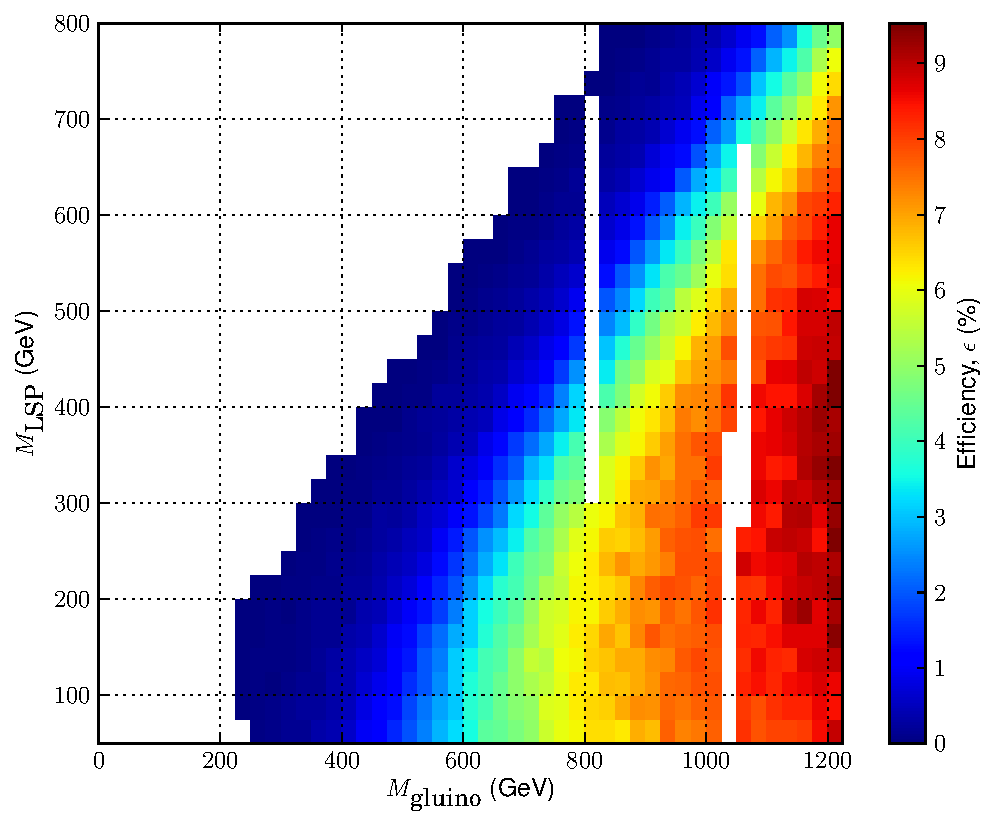
\includegraphics[width=0.49\textwidth]{fig/t3w_0p75_muons_eff_total}}
\subfloat[\Pe, $x=0.25$]{\label{fig:inter_t3w_el_efftot}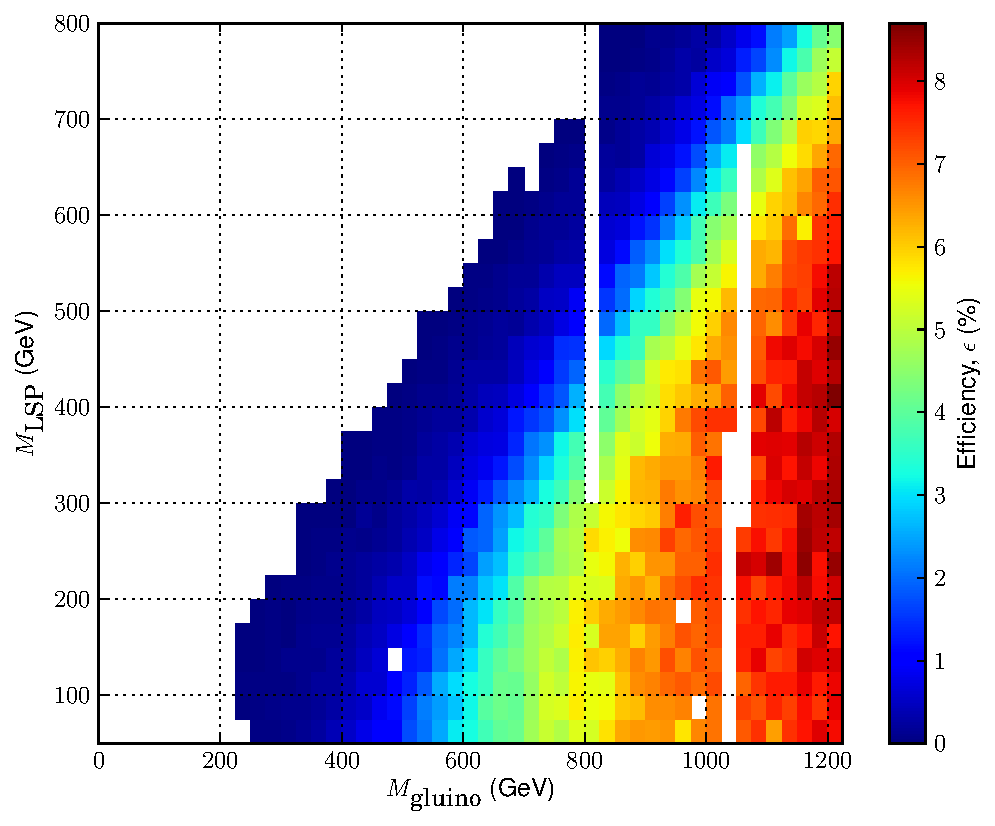
\includegraphics[width=0.49\textwidth]{fig/t3w_0p75_electrons_eff_total}}\\
\subfloat[\Pmu, $x=0.5$]{\label{fig:inter_t3w_mu_efftot}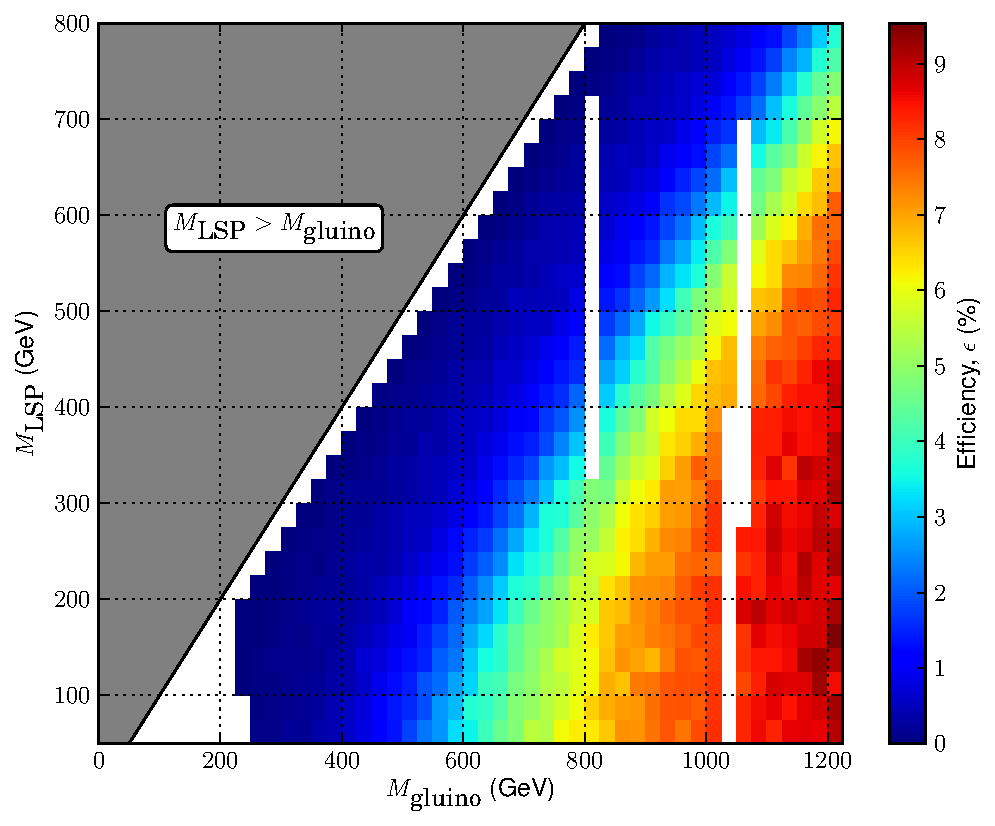
\includegraphics[width=0.49\textwidth]{fig/t3w_0p50_muons_eff_total}}
\subfloat[\Pe, $x=0.5$]{\label{fig:inter_t3w_el_efftot}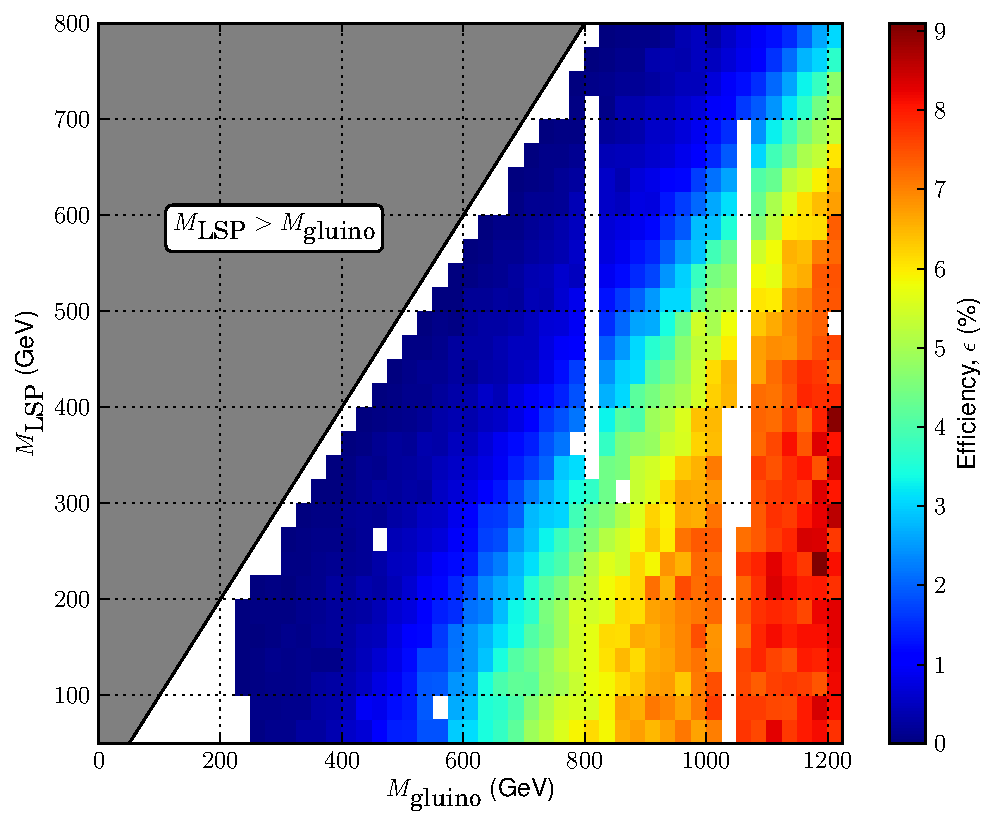
\includegraphics[width=0.49\textwidth]{fig/t3w_0p50_electrons_eff_total}}\\
\subfloat[\Pmu, $x=0.75$]{\label{fig:inter_t3w_mu_efftot}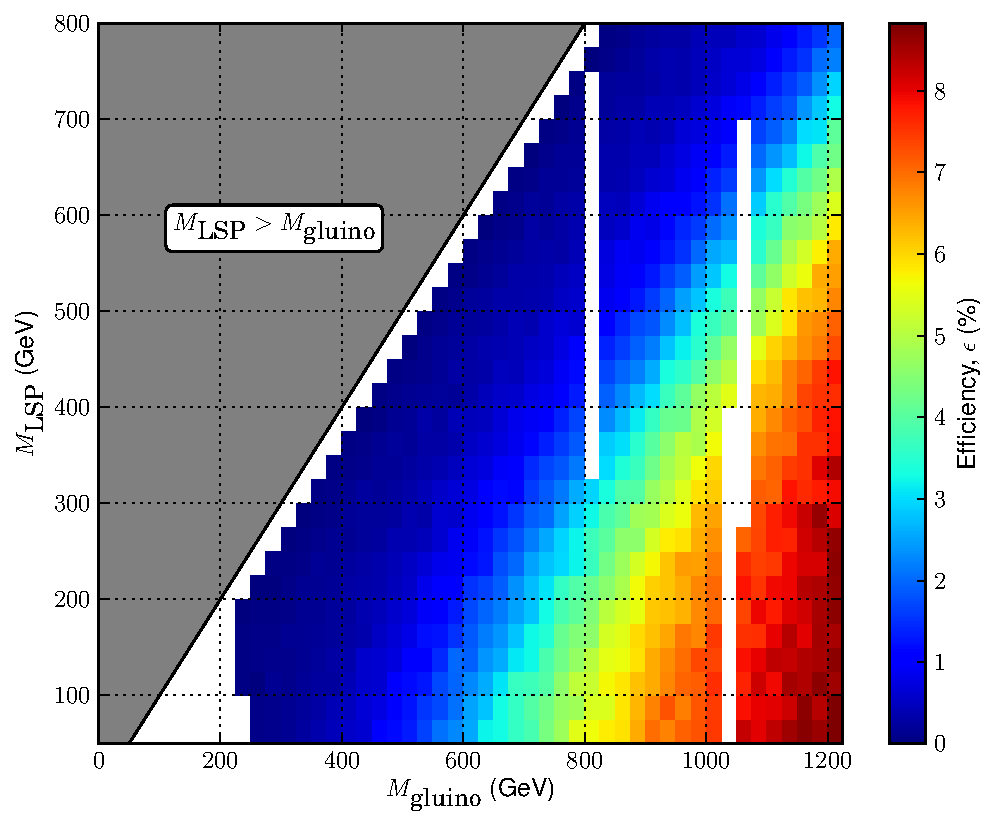
\includegraphics[width=0.49\textwidth]{fig/t3w_0p25_muons_eff_total}}
\subfloat[\Pe, $x=0.75$]{\label{fig:inter_t3w_el_efftot}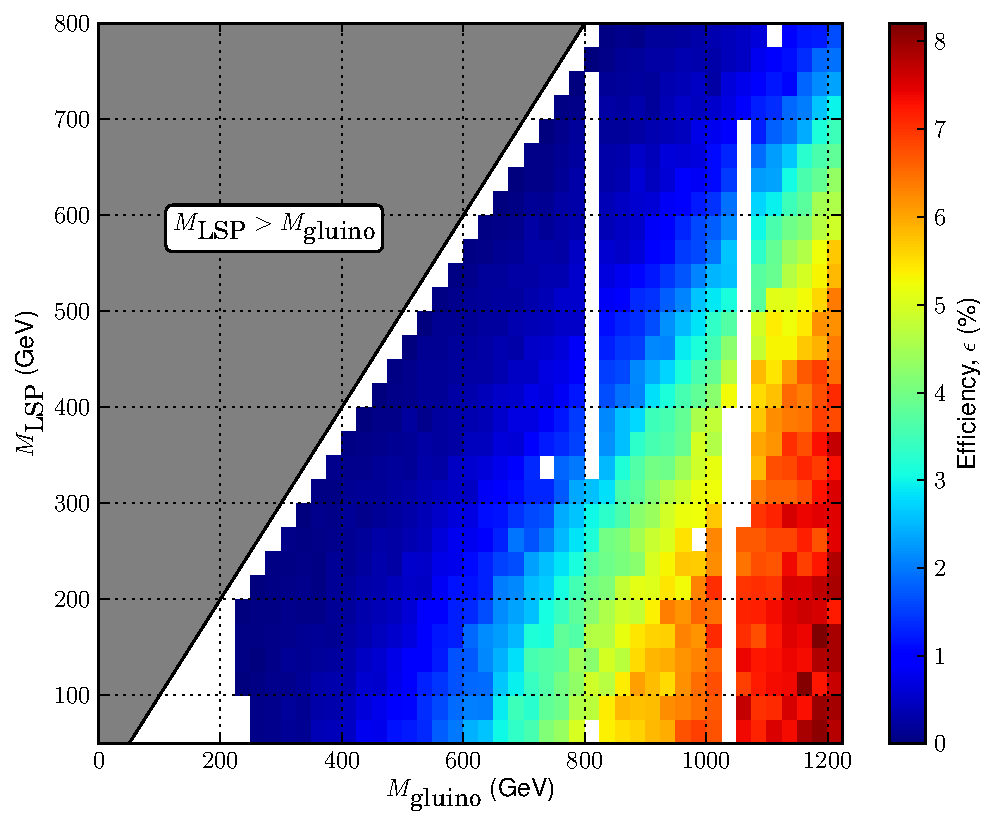
\includegraphics[width=0.49\textwidth]{fig/t3w_0p25_electrons_eff_total}}
\caption[Plots of total signal efficiency for muon and electron channels in
\TthreeW simplified mode]{Plots of total signal efficiency for muon and electron
  channels in \TthreeW simplified model. Each plot shows efficiency as a function
  of $(\Mgluino, \Mlsp)$ for a given value of \Mchargino.}
\label{fig:inter_t3w_eff}
\end{figure}

The observed limits for the each value of $x$ (0.25, 0.5 and 0.75) are shown in
Figures~\ref{fig:inter_t3w_0p75}, \ref{fig:inter_t3w_0p50} and
\ref{fig:inter_t3w_0p25} respectively. The exclusion is with respect to a
refernce cross-section for squark production calculated assuming
\ac{QCD}-strength couplings.

% TODO: Alex needs to check this weirdness!!
Comparing the exclusion contours, there does not appear to be a strong
dependence on \Mchargino. The reach of the search can be seen to improve
slightly for lower values of $x$ when the mass splitting between the mother and
the \ac{LSP} is reasonably large. From Eqn~\ref{eqn:tthreew_x}, these models
have an intermediate particle with a mass closer to the \ac{LSP} than to the
mother. In such events, the \PW would be expected to be relatively soft and the
jets from the cascade hard. With respect to the analysis selection, the
efficiency of the \HT cut would be expected to increase. On the other hand, for
a softer \PW, the \STlep efficiency may decrease due to the smaller charged
lepton momentum. Overall, the second effect is likely to be small since \STlep
is likely to be dominated by the missing energy from the \acp{LSP}.

In the cases where the mass splitting between mother and \ac{LSP} is smaller,
models with \Mchargino close to \Mgluino appears to give better exclusion. In
these cases, one might guess that the harder \PW is more relevant has a greater
effect on the efficiency since there is less hadronic energy available from the
cascade.

% TODO: more spiel here

\begin{figure}[h!]
\centering
\subfloat[]{\label{fig:inter_t3w_0p25_limit}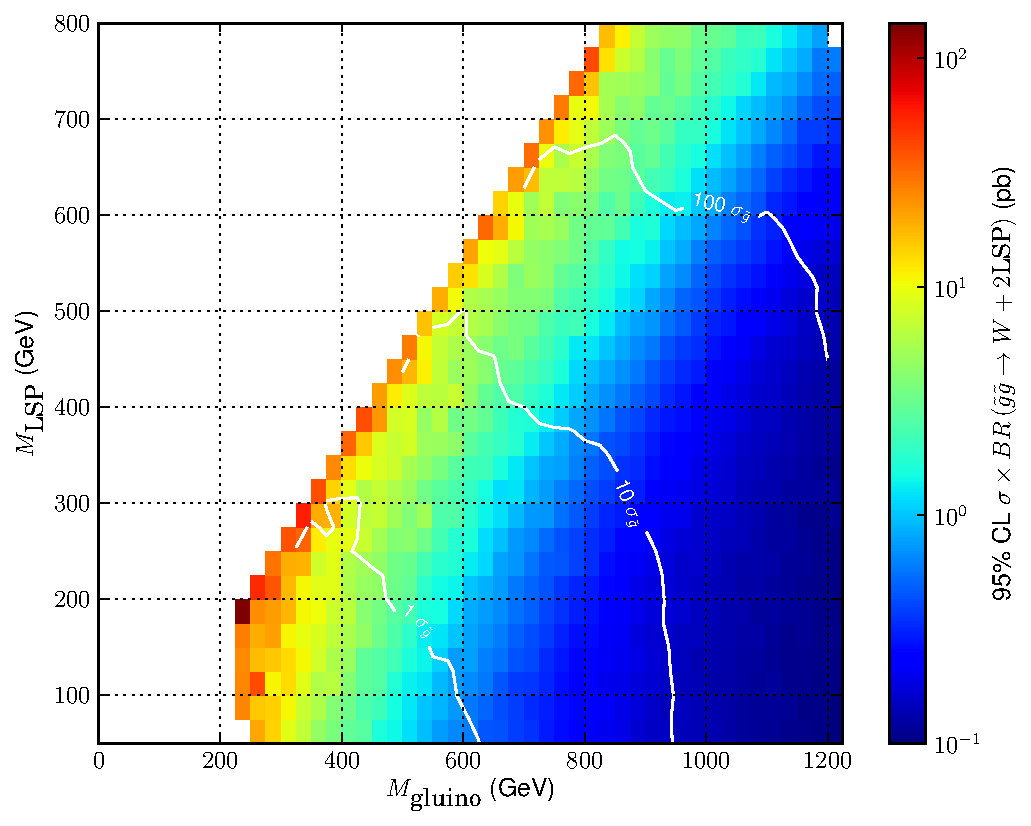
\includegraphics[width=0.49\textwidth]{fig/t3w_0p25_limit}}
\subfloat[]{\label{fig:inter_t3w_0p25_limit_1d}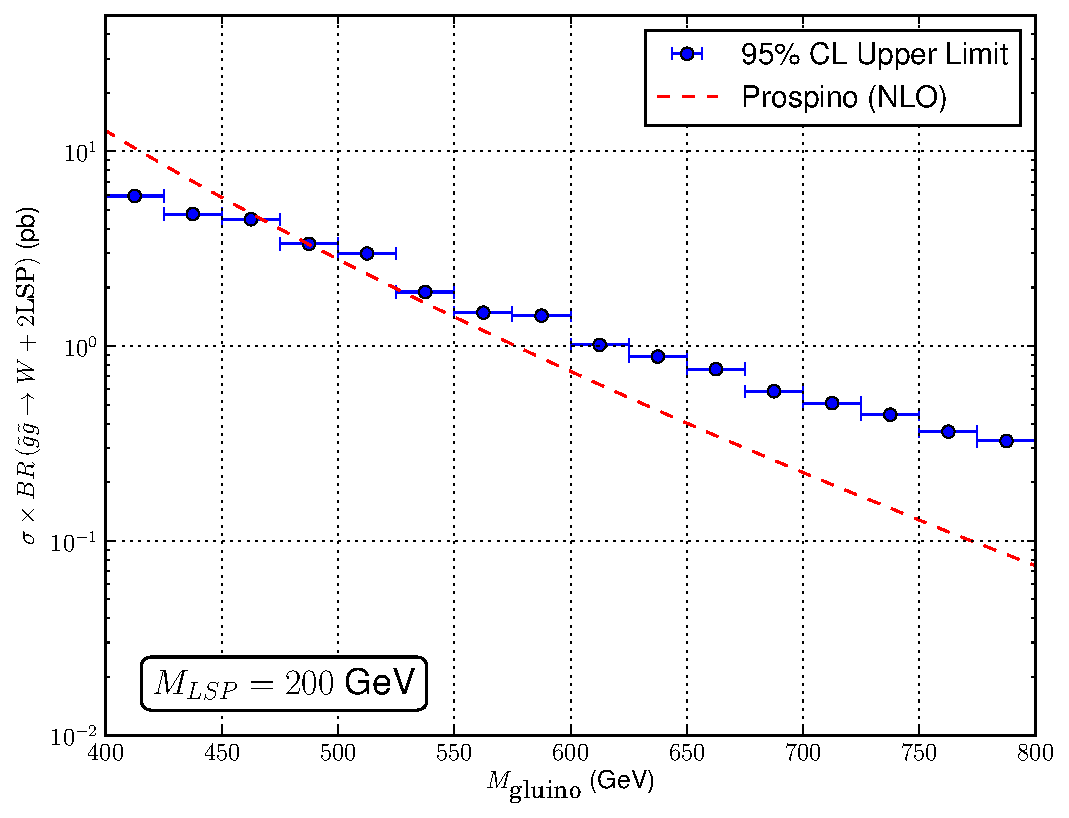
\includegraphics[width=0.49\textwidth]{fig/t3w_0p25_limit_1d}}
\caption[Limits for the \TthreeW simplified model with \Mchargino set assuming
$x=0.75$]{Limits for the \TthreeW simplified model with \Mchargino set assuming
  $x=0.75$. The 95\% confidence level upper limit on the cross-section as a
  function of $(\Mgluino, \Mlsp$) is shown in
  \subref{fig:inter_t3w_0p25_limit}. Overlayed are contours showing this
  exclusion in terms 1, 10 or 100 times the gluino cross-section predicted by
  \ac{QCD}. Figure \subref{fig:inter_t3w_0p25_limit_1d} shows the same upper
  limit as a function of \Mgluino with $\Mlsp = \unit{50}{\GeV}$. Overlayed is
  the \ac{QCD} cross-section for gluino production.}
\label{fig:inter_t3w_0p25}
\end{figure}

\begin{figure}
\centering
\subfloat[]{\label{fig:inter_t3w_0p50_limit}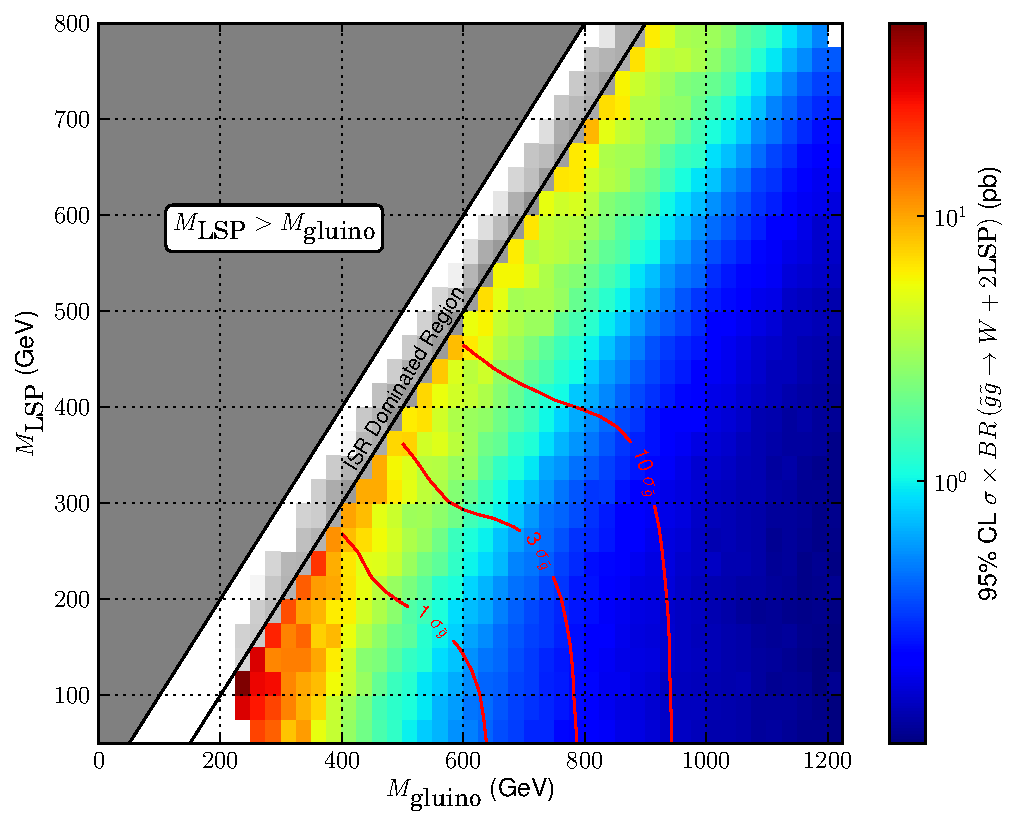
\includegraphics[width=0.49\textwidth]{fig/t3w_0p50_limit}}
\subfloat[]{\label{fig:inter_t3w_0p50_limit_1d}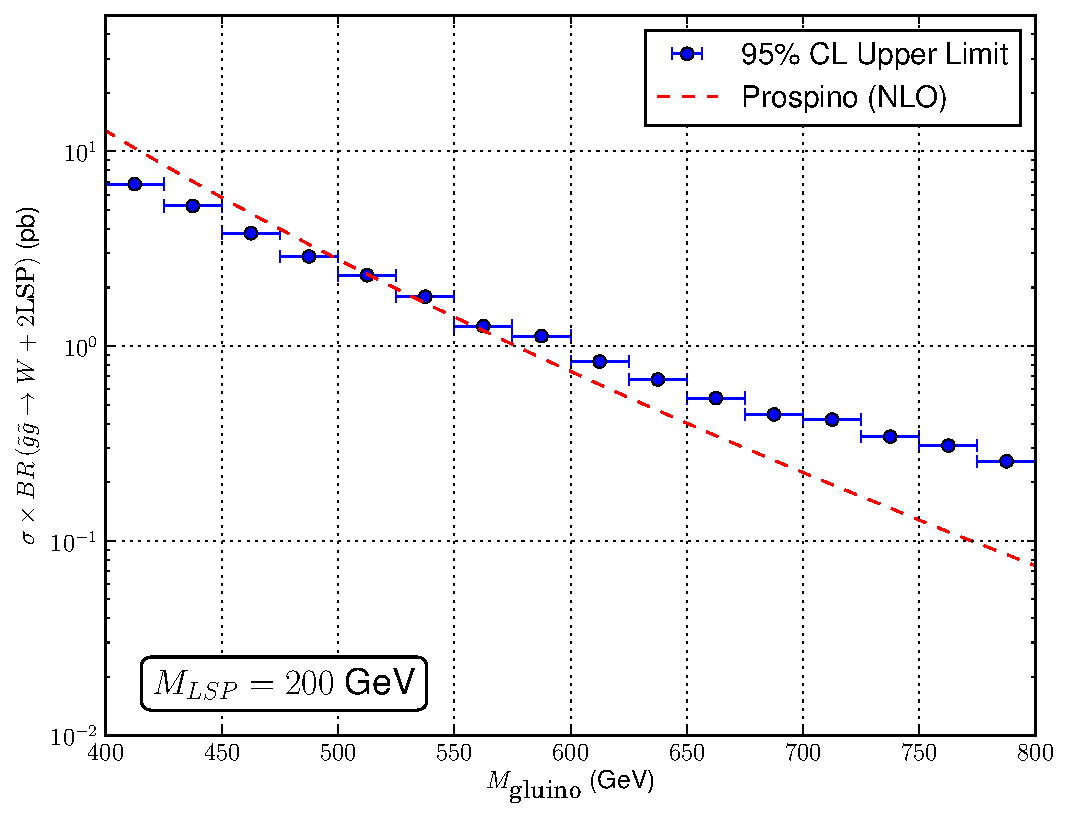
\includegraphics[width=0.49\textwidth]{fig/t3w_0p50_limit_1d}}
\caption[Limits for the \TthreeW simplified model with \Mchargino set assuming
$x=0.5$]{Limits for the \TthreeW simplified model with \Mchargino set assuming
  $x=0.5$. The 95\% confidence level upper limit on the cross-section as a
  function of $(\Mgluino, \Mlsp$) is shown in
  \subref{fig:inter_t3w_0p25_limit}. Overlayed are contours showing this
  exclusion in terms 1, 10 or 100 times the gluino cross-section predicted by
  \ac{QCD}. Figure \subref{fig:inter_t3w_0p25_limit_1d} shows the same upper
  limit as a function of \Mgluino with $\Mlsp = \unit{50}{\GeV}$. Overlayed is
  the \ac{QCD} cross-section for gluino production.}
\label{fig:inter_t3w_0p50}
\end{figure}

\begin{figure}
\centering
\subfloat[]{\label{fig:inter_t3w_0p75_limit}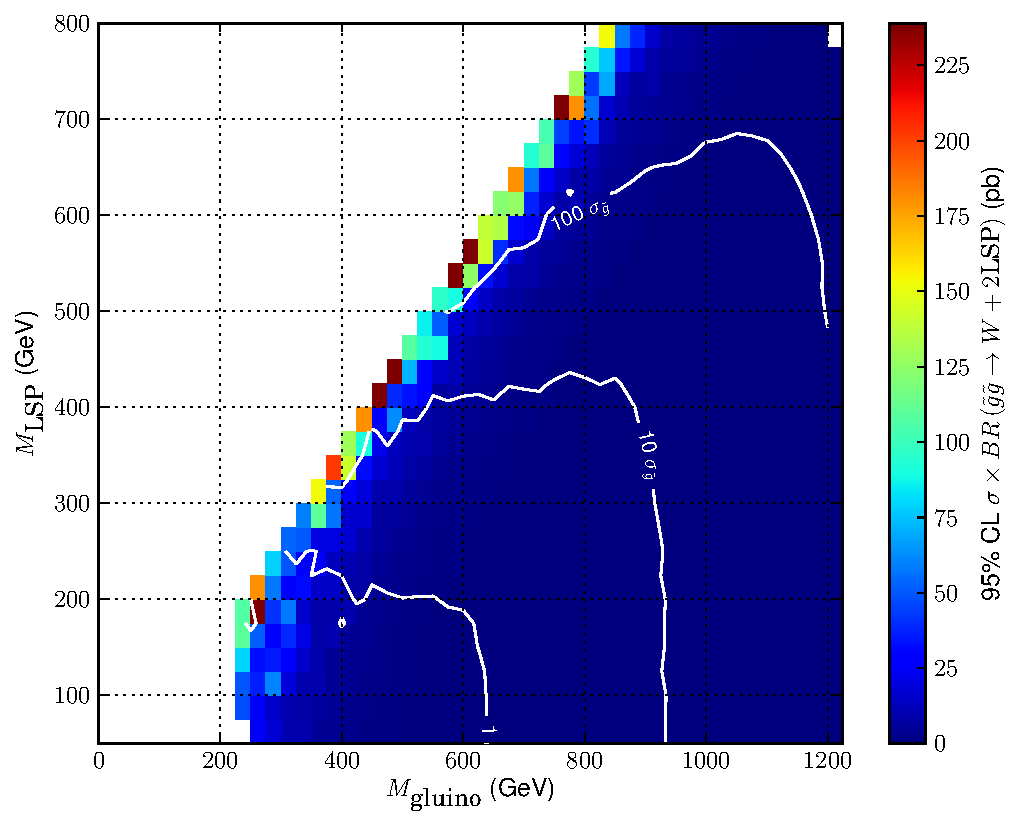
\includegraphics[width=0.49\textwidth]{fig/t3w_0p75_limit}}
\subfloat[]{\label{fig:inter_t3w_0p75_limit_1d}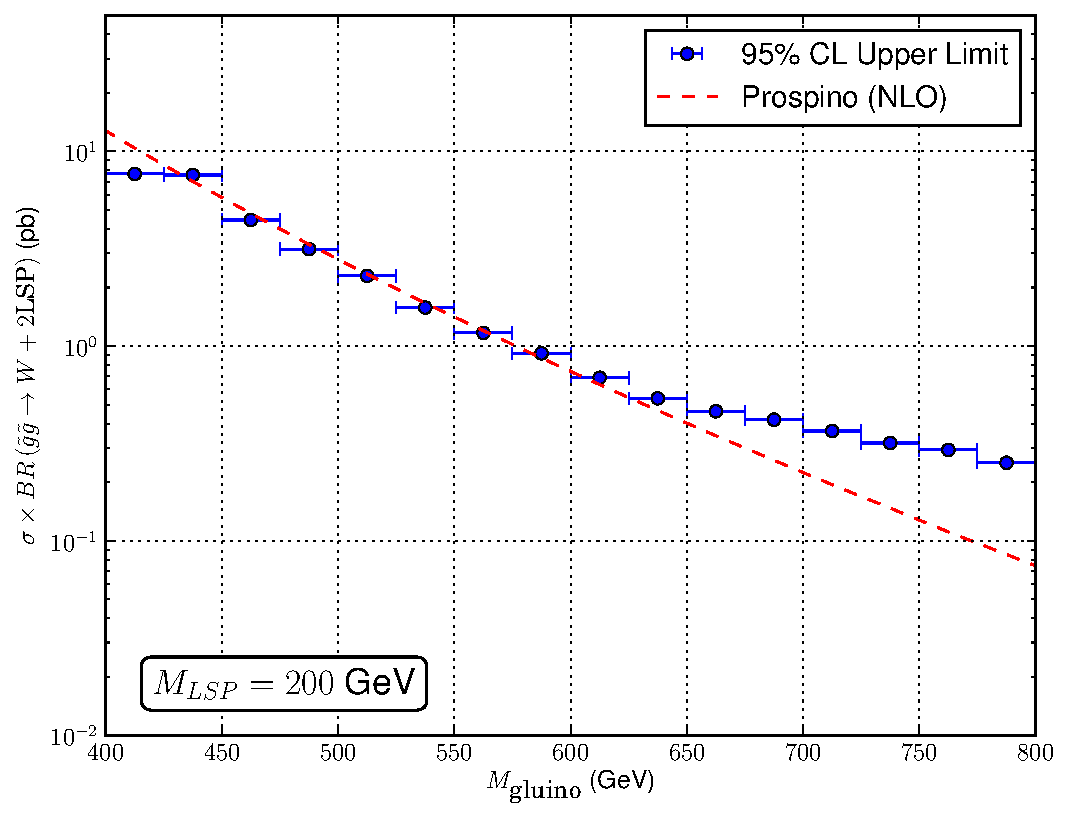
\includegraphics[width=0.49\textwidth]{fig/t3w_0p75_limit_1d}}
\caption[Limits for the \TthreeW simplified model with \Mchargino set assuming
  $x=0.25$]{Limits for the \TthreeW simplified model with \Mchargino set assuming
  $x=0.25$. The 95\% confidence level upper limit on the cross-section as a
  function of $(\Mgluino, \Mlsp$) is shown in
  \subref{fig:inter_t3w_0p25_limit}. Overlayed are contours showing this
  exclusion in terms 1, 10 or 100 times the gluino cross-section predicted by
  \ac{QCD}. Figure \subref{fig:inter_t3w_0p25_limit_1d} shows the same upper
  limit as a function of \Mgluino with $\Mlsp = \unit{50}{\GeV}$. Overlayed is
  the \ac{QCD} cross-section for gluino production.}
\label{fig:inter_t3w_0p75}
\end{figure}

\subsubsection{\Ttwott}
The \Ttwott model, as previously discussed, is of theoretical interest for
describing \ac{SUSY} theories with light stop squarks.

Efficiencies for each point in the $(\Mstop, \Mlsp)$ plane are shown in
Figures~\ref{fig:inter_t2tt_mu} and \ref{fig:inter_t2tt_el} for muons and
electrons respectively. Efficiencies are shown per \STlep bin in order to gauge
the effect of this cut on the efficiency.

\begin{figure}[h!]
\centering
\subfloat[$250 < \STlep < 350$]{\label{fig:inter_t2tt_mu_eff250}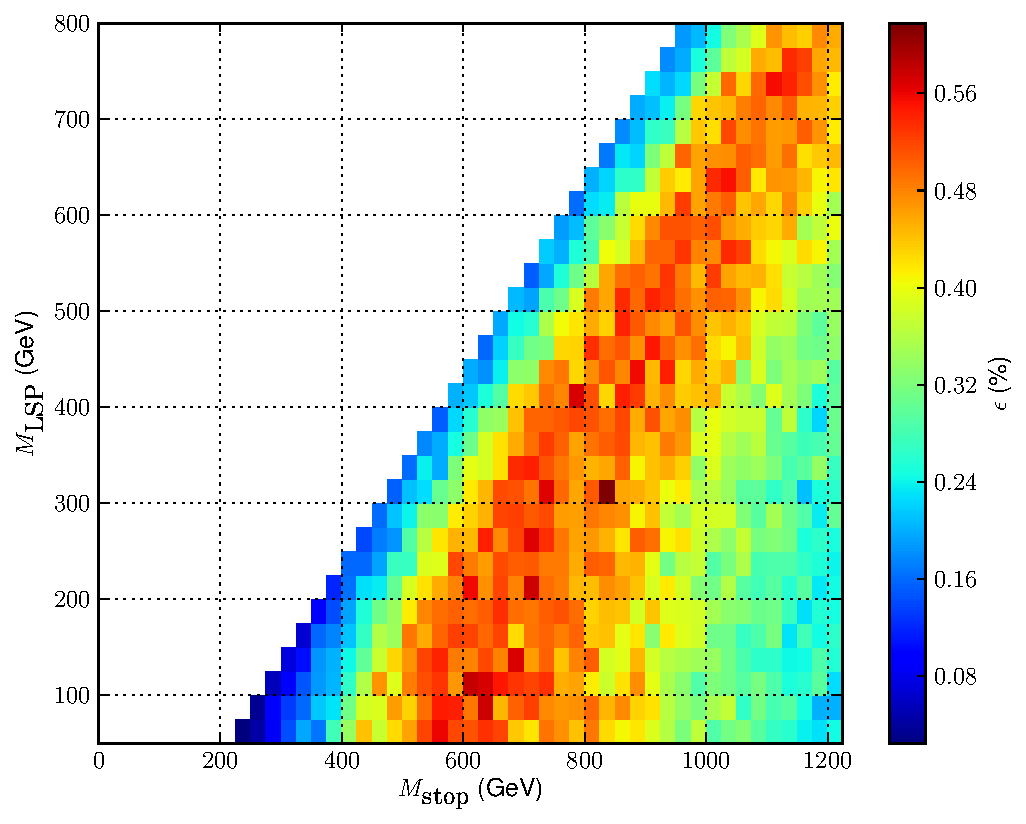
\includegraphics[width=0.49\textwidth]{fig/t2tt_muons_eff_250}}
\subfloat[$350 < \STlep < 450$]{\label{fig:inter_t2tt_mu_eff350}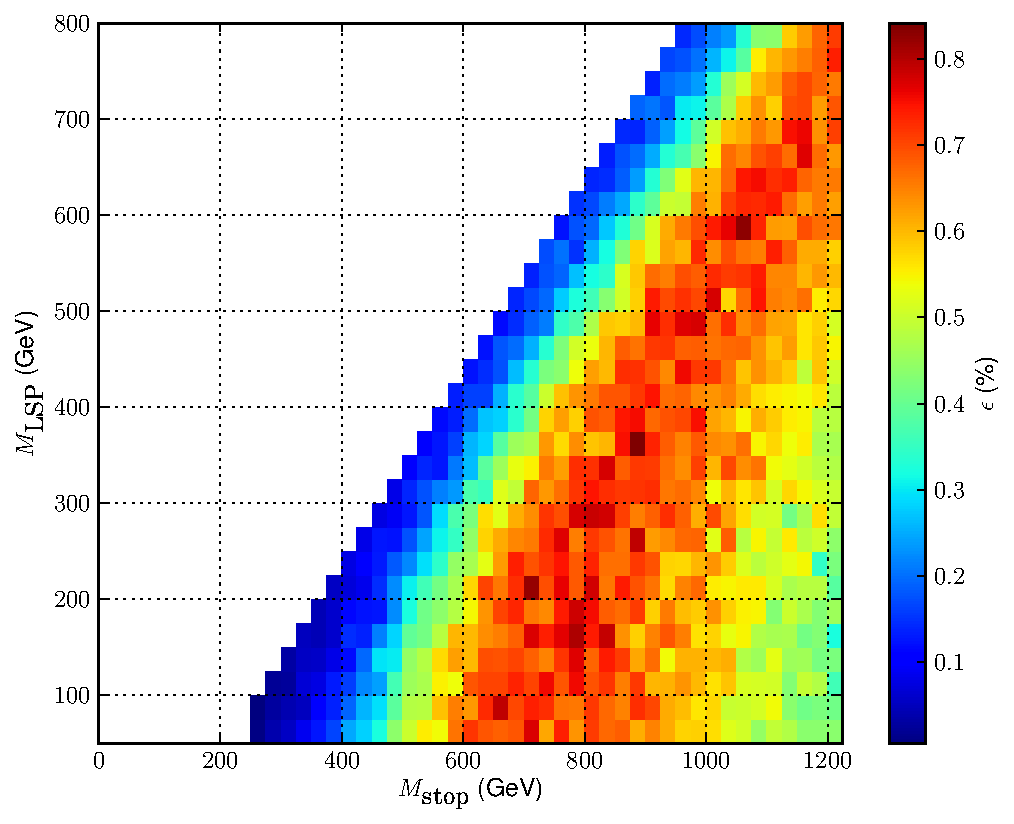
\includegraphics[width=0.49\textwidth]{fig/t2tt_muons_eff_350}}\\
\subfloat[$\STlep > 450$]{\label{fig:inter_t2tt_mu_eff450}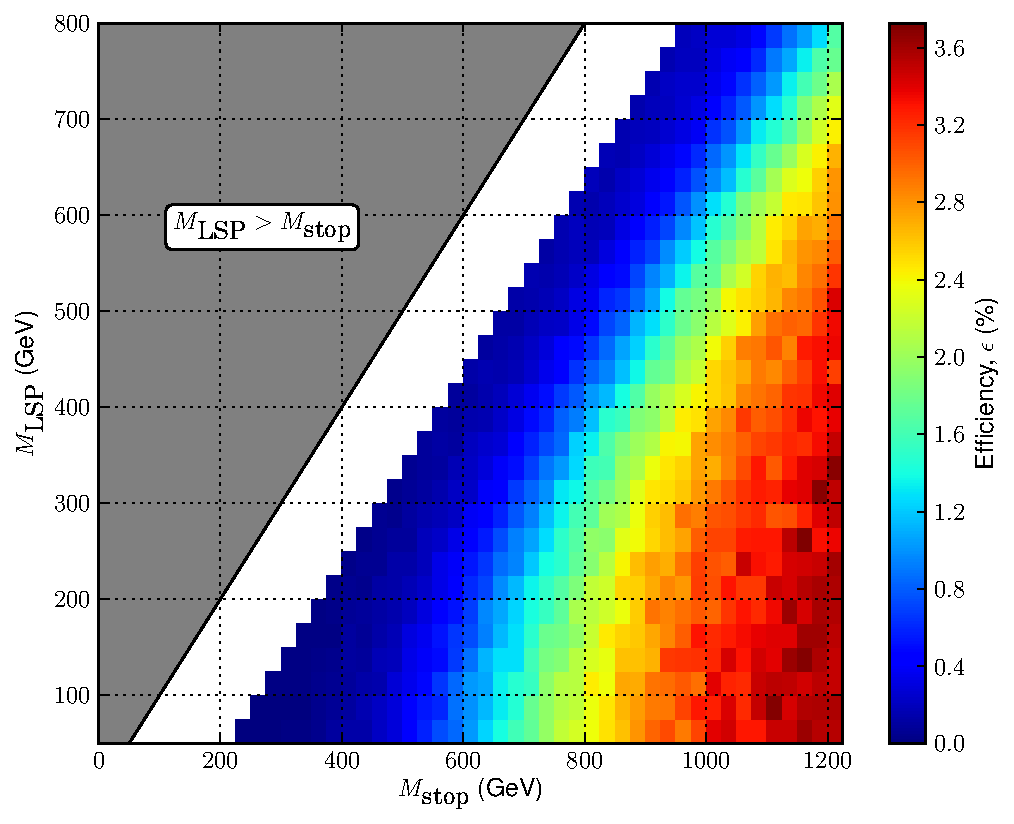
\includegraphics[width=0.49\textwidth]{fig/t2tt_muons_eff_450}}
\subfloat[Total]{\label{fig:inter_t2tt_mu_efftot}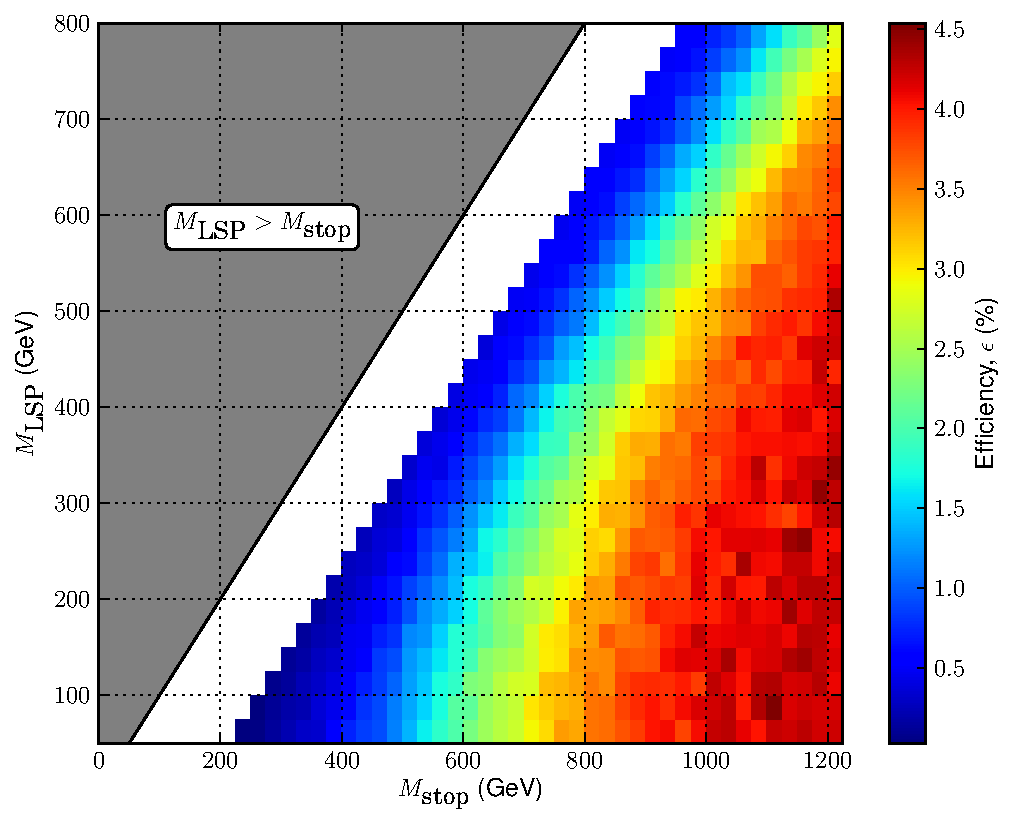
\includegraphics[width=0.49\textwidth]{fig/t2tt_muons_eff_total}}
\caption[Signal efficiency maps for the muon channel in the \Ttwott simplified
  model]{Signal efficiency maps for the muon channel in the \Ttwott simplified
  model. Efficiency is shown as a function of $(\Mstop, \Mlsp)$ for each \STlep
  bin and for the total across all three bins.}
\label{fig:inter_t2tt_mu}
\end{figure}

\begin{figure}[h!]
\centering
\subfloat[$250 < \STlep < 350$]{\label{fig:inter_t2tt_el_eff250}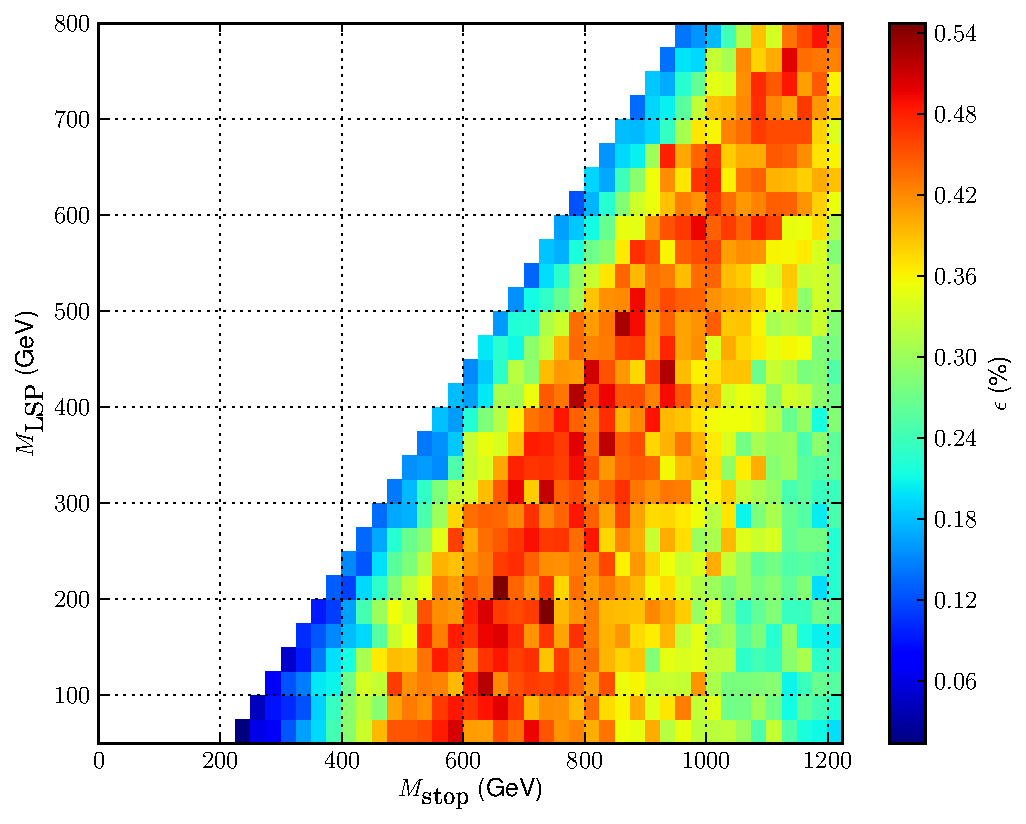
\includegraphics[width=0.49\textwidth]{fig/t2tt_electrons_eff_250}}
\subfloat[$350 < \STlep < 450$]{\label{fig:inter_t2tt_el_eff350}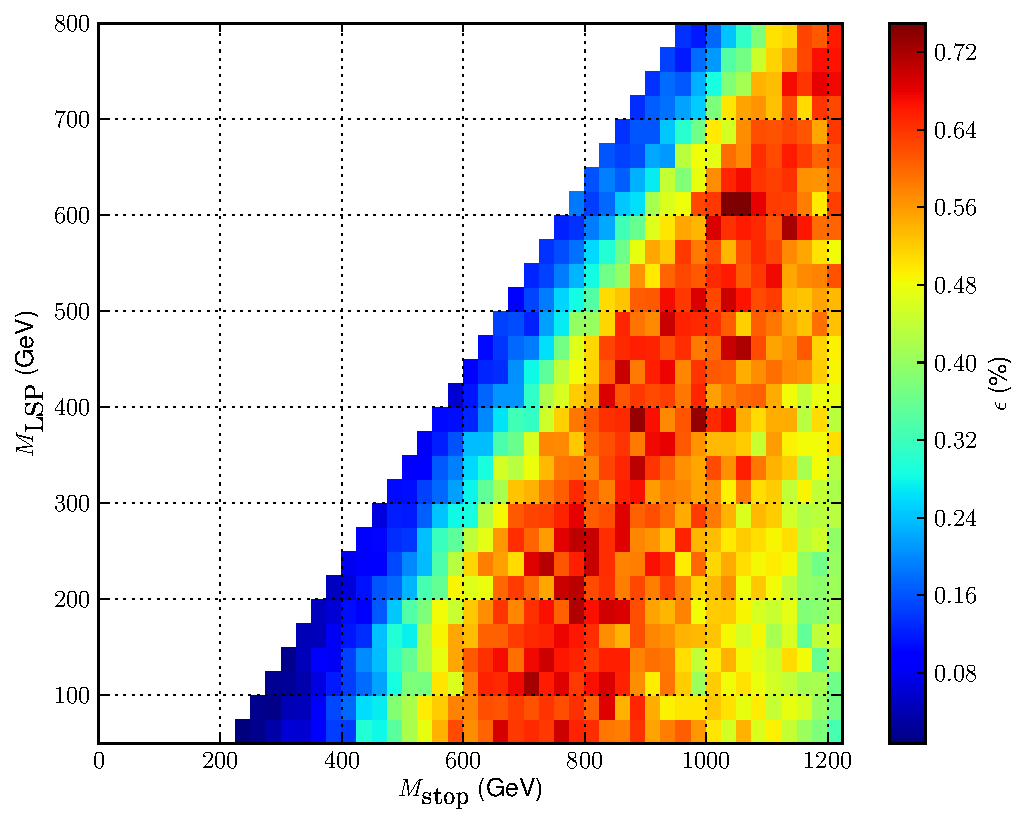
\includegraphics[width=0.49\textwidth]{fig/t2tt_electrons_eff_350}}\\
\subfloat[$\STlep > 450$]{\label{fig:inter_t2tt_el_eff450}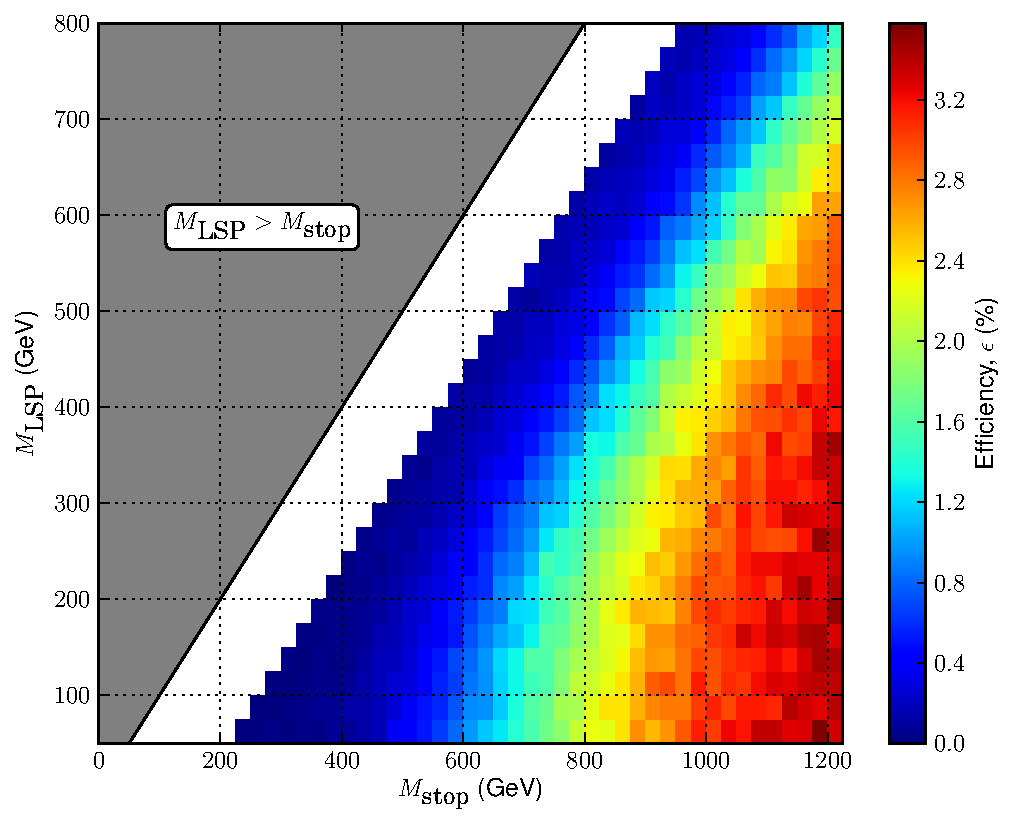
\includegraphics[width=0.49\textwidth]{fig/t2tt_electrons_eff_450}}
\subfloat[Total]{\label{fig:inter_t2tt_el_efftot}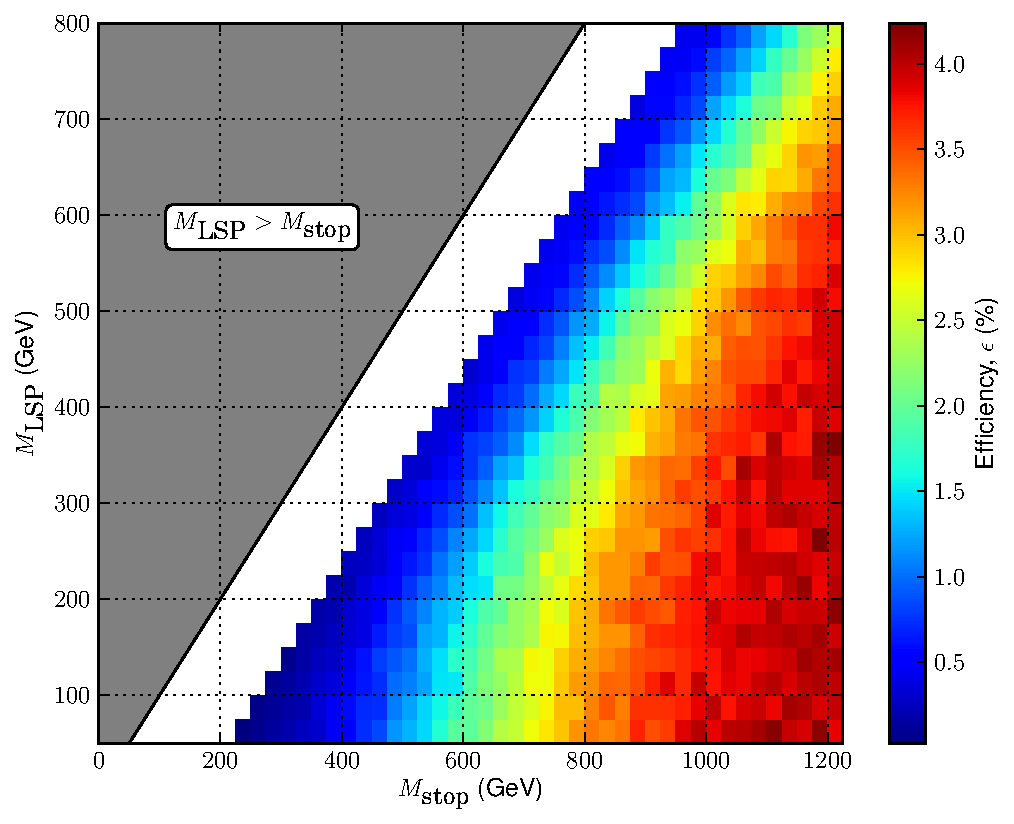
\includegraphics[width=0.49\textwidth]{fig/t2tt_electrons_eff_total}}
\caption[Signal efficiency maps for the electron channel in the \Ttwott simplified
  model]{Signal efficiency maps for the electron channel in the \Ttwott simplified
  model. Efficiency is shown as a function of $(\Mstop, \Mlsp)$ for each \STlep
  bin and for the total across all three bins.}
\label{fig:inter_t2tt_el}
\end{figure}

The observed limit is shown in a similar fashion to the \TthreeW case in
Figure~\ref{fig:inter_t2tt}. It can be seen that very little exclusion is
achieved with respect to the stop cross-section predicted from \ac{QCD}. It is
possible that a dedicated search using B-tagged jets would provide significantly
improved sensitivity.

\begin{figure}[h!]
\centering
\subfloat[]{\label{fig:inter_t2tt_limit}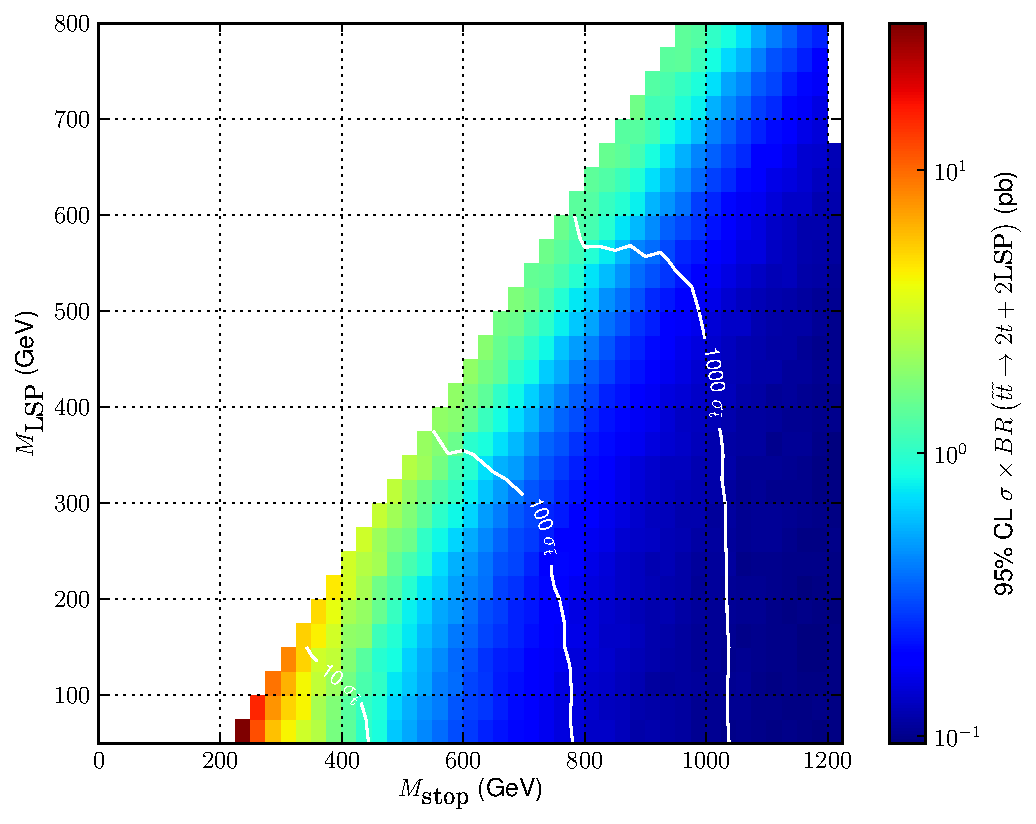
\includegraphics[width=0.49\textwidth]{fig/t2tt_limit}}
\subfloat[]{\label{fig:inter_t2tt_limit_1d}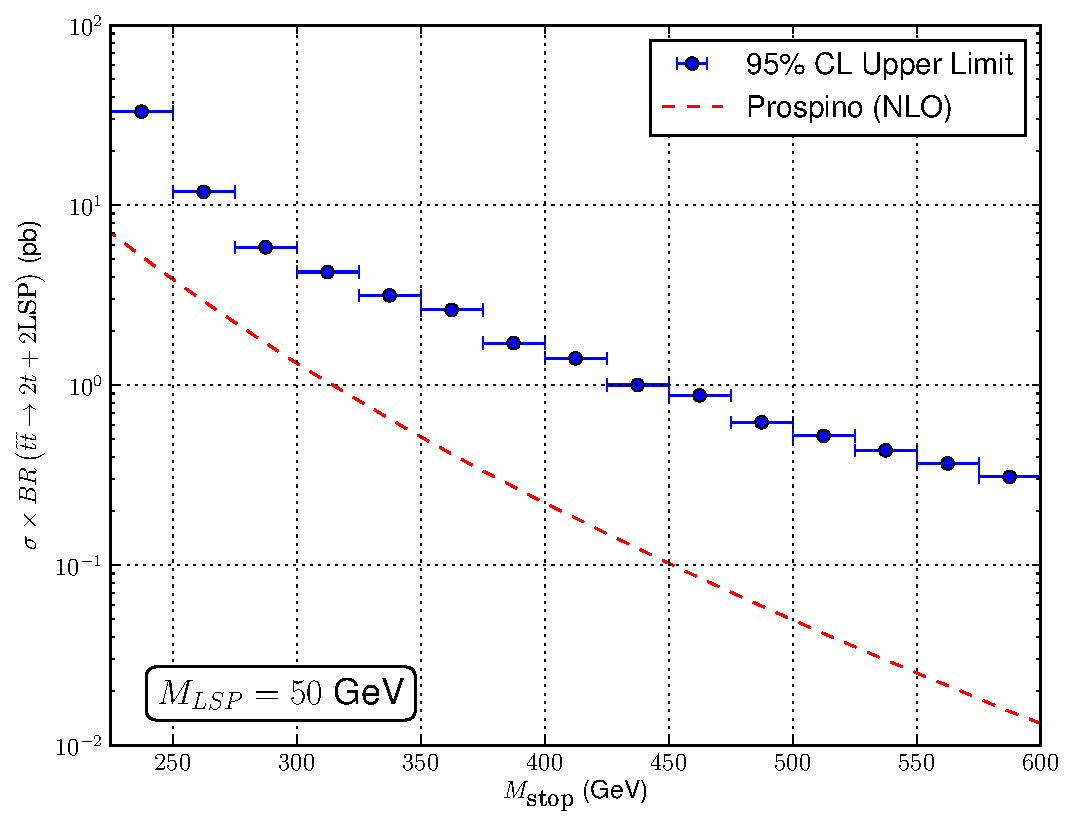
\includegraphics[width=0.49\textwidth]{fig/t2tt_limit_1d}}
\caption[]{95\% upper limit on the cross-section for the \Ttwott simplified
  model. The two-dimensional plot \subref{fig:inter_t2tt_limit} shows the upper
  limit as a function of $(\Mstop, \Mlsp)$. The contours overlayed show this
  exclusion in terms of 1, 10 and 1000 times the stop production cross-section
  predicted by \ac{QCD}. The upper limit is shown as a function of \Mstop in
  \subref{fig:inter_t2tt_limit_1d} for $\Mlsp = \unit{50}{\GeV}$. }
\label{fig:inter_t2tt}
\end{figure}





%%% Local Variables:
%%% mode: latex
%%% TeX-master: "../thesis"
%%% End:
